\documentclass{mythesis}
\usepackage{mythesis}

%% You can set the line spacing this way
%\setallspacing{double}
%% or a section at a time like this
%\setfrontmatterspacing{double}

%% PDF metadata
\makeatletter
\@ifpackageloaded{hyperref}{%
\hypersetup{%
pdftitle = {Studying B to K pi decays with LHCb},
pdfsubject = {Andy Buckley's PhD thesis},
pdfkeywords = {LHCb, B, physics, LHC, heavy flavour},
pdfauthor = {\textcopyright\ Andy Buckley}
}
}{}
\makeatother

%% Define the thesis title and author
\title{Searching for Supersymmetry in the Single Lepton Channel at CMS Using Helicity Polarisation Methods} \author{Alexander Sparrow}

%% Start the document
\begin{document}

\begin{acronym}
\acro{NP}{New Physics}
\acro{SM}{Standard Model}
\acro{ALICE}{A Large Ion Collider Experiment}
\acro{ATLAS}{A Toroidal LHC Apparatus}
\acro{LHCb}{Large Hadron Collider Beauty Experiment}
\acro{TOTEM}{Total Elastic and diffractive cross section Measurement}
\acro{LHCf}{Large Hadron Collider Forward}
\acro{CMS}{Compact Muon Solenoid}
\acro{LHC}{Large Hadron Collider}
\acro{CERN}{Conseil Européen pour la Recherche Nucléaire}
\acro{LEP}{Large Electron-Positron Collider}
\acro{PSB}{Proton Synchrotron Booster}
\acro{PS}{Proton Synchrotron}
\acro{SPS}{Super Proton Synchrotron}
\acro{LEIR}{Low Energy Ion Storage Ring}
\acro{ECAL}{Electromagnetic Calorimeter}
\acro{HCAL}{Hadronic Calorimeter}
\acro{HE}{Hadronic Calorimeter Endcap}
\acro{HB}{Hadronic Calorimeter Barrel}
\acro{CSC}{Cathode Strip Chambers}
\acro{DT}{Drift Tubes}
\acro{EB}{ECAL Barrel}
\acro{EE}{ECAL Endcap}
\acro{TIB}{Tracker Inner Barrel}
\acro{TOB}{Tracker Outer Barrel}
\acro{TID}{Tracker Inner Disk}
\acro{TEC}{Tracker Endcap}
\acro{APD}{Avalanche Photodiode}
\acro{VPT}{Vacuum Phototriode}
\acro{SUSY}{Supersymmetry}
\acro{CMSSM}{Constrained Minimal Supersymmetric Standard Model}
\acro{mSUGRA}{Minimal Supergravity}
\acro{GMSB}{Gauge-Mediated Supersymmetry Breaking}
\acro{LSP}{Lightest Supersymmetric Particle}
\acro{WIMP}{Weakly Interacting Massive Particle}
\end{acronym}

%% Define the un-numbered front matter (cover pages, rubrik and table of contents)
\begin{frontmatter}
  %% Title
\titlepage[of Imperial College London]%
{A dissertation submitted to Imperial College London\\
 for the degree of Doctor of Philosophy}

\input{status.tex}

%% Abstract
\begin{abstract}%[\smaller \thetitle\\ \vspace*{1cm} \smaller {\theauthor}]
  %\thispagestyle{empty}
  Abstract to go here
\end{abstract}


%% Declaration
\begin{declaration}
  This dissertation is the result of my own work, except where explicit
  reference is made to the work of others, and has not been submitted
  for another qualification to this or any other university.

  The work presented in Chapters~\ref{sec:wpol}, \ref{sec:susysearch},
  \ref{sec:interpretation} is the result of collaboration with a number of
  others. For completeness and necessary context, I have presented a full
  account of these analyses. For the \PW polarisation measurement, my
  contributions were primarily to the electron channel measurement and the
  fitting procedure. For the supersymmetry search, I worked mostly on the
  estimation of the systematic uncertainties and optimising some of the
  selection cuts. I also set up the statistics procedure detailed in
  Appendix~\ref{sec:inter_1lepton} and performed the interpretation and
  validation work shown in Chapter~\ref{sec:interpretation}.

  \vspace*{1cm}
  \begin{flushright}
    Alexander Sparrow
  \end{flushright}
\end{declaration}


%% Acknowledgements
\begin{acknowledgements}
  Of the many people who deserve thanks, some are particularly prominent,
  such as my supervisor\dots
\end{acknowledgements}


%% Preface
\begin{preface}
  This thesis describes my research on various aspects of the \LHCb
  particle physics program, centred around the \LHCb detector and \LHC
  accelerator at \CERN in Geneva. Waaay!

  \noindent
  % for this example, I'll just mention \ChapterRef{chap:SomeStuff}
  % and \ChapterRef{chap:MoreStuff}.
\end{preface}

%% ToC
\tableofcontents

\listoffigures
\listoftables

%% Strictly optional!
\frontquote%
{Time is a companion that goes with us on a journey. It reminds us to cherish
  each moment, because it will never come again. What we leave behind is not as
  important as how we have lived.}%
{Jean-Luc Picard, 2371, after the destruction of the Enterprise-D}

\end{frontmatter}
%% Start the content body of the thesis
\begin{mainmatter}
  \linenumbers
  %% Actually, more semantic chapter filenames are better, like "chap-bgtheory.tex"
  \import{1-sm/}{sm}
  \import{2-susy/}{susy}
  \import{3-expt/}{expt}
  \import{4-reco/}{reco}
  \import{5-wpol/}{wpol}
  \import{6-susysearch/}{susysearch}
  \import{7-interpretation/}{interpretation}

  %% To ignore a specific chapter while working on another,
  %% making the build faster, comment it out like this:
  %\input{chap4}
  \nolinenumbers
\end{mainmatter}

%% AS: Added to make scons seen these files (it doesn't parse the import
%% statements above!)
\begin{comment}
  \chapter{The Standard Model}
\label{sec:sm}
\section{Introduction}
The \acl{SM} of particle physics is the best available theory describing the
interactions of all known fundamental particles. It is perhaps the most
extensively tested of any fundamental theory of nature, having withstood the
scrutiny of several decades of data-taking at a number of large, high-energy
physics experiments. However, despite this success, there appear to be a number
of major theoretical deficiencies in desperate need of attention. In this
chapter, the foundations of the theory will be laid out in a concise manner. The
aforementioned theoretical difficulties will be described in detail. This will
serve to motivate the potential solutions offered by the following chapter, and
ultimately the analysis work that has been undertaken.

It is important to note that, although the \ac{SM} will be presented here as a
complete theory, seemingly designed to match the currently observed set of
fundamental particles, this is not how it came into being. The theory was built
up over much of the second half of the 20th centry and actually successfully
predicited a number of discoveries. Perhaps the best example of this is the
discovery of the \PW and \PZ bosons by the \ac{UA1} and \ac{UA2} experiments at
\ac{CERN} in 1983. These had been theorised by Weinberg, Glashow and Salam in
1968.

\section{Particles and Fundamental Forces}
\label{sec:theory:particles}
The \ac{SM} represents the unification of three of the four known fundamental
forces, namely: electromagnetism, the weak nuclear force and the strong nuclear
force. The other force, gravity, having resisted unification with the other
three, is not part of the \ac{SM}.

Within the \ac{SM}, each fundamental force is mediated by one or more ``gauge
bosons''. For electromagnetism, this is the photon, for the weak force, the
\PWp, \PWm and \PZ. Strong interactions are believed to be mediated by a set of
8 ``gluons'' (\Pg). Each boson is a vector particle and thus has a spin of 1.

In addition to the bosons, the \ac{SM} must of course catalogue the many matter
particles discovered by experiment. These are the fermions and may be further
subdivided into leptons and quarks. The leptons, or ``light particles'' may be
divided into three generations. Each generation associates a relatively heavy
charged lepton with a much lighter neutral partner, referred to as a
neutrino. The charged leptons are: the electron (\Pe), the muon (\Pgm) and the
tau lepton (\Ptau). Each has the same charge, typically written in terms of the
charge carried by a single electron, \ec. The corresponding neutrinos are then
referred to as the electron neutrino (\Pnue), muon neutrino (\Pnum) and tau
neutrino (\Pnut) respectively.

The quarks also appear to occupy three generations, with two quarks occupying
each. The first of each generation is referred to as an ``up-type'' quark and
has charge $+\frac{2}{3}\ec$, the second ``down-type'' with charge
$-\frac{1}{3}\ec$. The up-type quarks are (in order of increasing mass): up
(\Pup), charm (\Pcharm) and top (\Ptop). Similarly, the respective down-type
partners are: down (\Pdown), strange (\Pstrange) and bottom\footnote{also known
  as beauty} (\Pbottom). In addition to electromagnetism and the weak force,
quarks interact via the strong nuclear force.

Each of the fermions is associated with an anti-particle partner, with opposite
charge. For the charged leptons, the charge may be indicated by a superscript,
e.g. \Pep, \Pem, \Pgmp, \Pgmm etc. For the quarks, the anti-particles will
normally be denoted \APup, \APdown etc. In the case of the neutrinos, being
electromagnetically neutral, the question of the nature of the anti-particles is
as yet unanswered. It is theoretically possible for a neutrino to be its own
anti-particle, $\Pnulepton = \APnulepton$. This would make the neutrino a
``Majorana Fermion'' and is an area of active experimental research.

The particle content and properties of the \ac{SM} seem, at first glance, to be
quite arbitrary. Why are there three forces? Why does the Weak sector have three
bosons, and the electromagnetic only one. Some of these questions may be
answered by constructing the \ac{SM} as a gauge theory. This will be outlined in
the next section.
\section{Electroweak Gauge Theory}
\subsection{Gauge Invariance}
The theoretical principle of gauge invariance can be seen in Maxwell's theory of
electromagnetism \cite{aitchison}. Recall that the electric (\emE) and magnetic (\emB) components
of the field may be written in terms of a vector potential (\emA) and a scalar
potential \emV as follows:
\begin{eqnarray}
\emB = \nablav \times \emA \\
\emE = -\nablav \emV - \frac{\partial \emA}{\partial t}
\end{eqnarray}
It can be seen that these equations do not relate a given (\emB, \emE) to unique
values of \emA and \emV. In particular, if the following transformations are
applied simulatenously to \emA and \emV, the values of \emB and \emE will be
unchanged,
\begin{eqnarray}
\emA \longrightarrow \emA + \nablav \chi \\
\emV \longrightarrow  \emV - \frac{\partial \chi}{\partial t}
\end{eqnarray}
where $\chi$ is some arbitrary function. Such transformations are known as
``gauge transformations'' and similarly \emB and \emE are said to be ``gauge
invariant''.

If the scalar and vector potentials are rewritten in terms of a single 4-vector
potential, $\Amu = (\emV, \emA)$ and similarly taking a 4-vector differntial
operator, $\dmu = (\partial/\partial t, -\nablav)$, the gauge transformation
takes the form
\begin{equation}
\Amu \longrightarrow \Amu - \dmu\chi
\label{eqn:theory_gauge_transform}
\end{equation}
In this form, the Maxwell equations can be rewritten as
\begin{equation}
\dmu \Fmunu = j^{\nu}_{\textrm{em}}
\end{equation}
where $\Fmunu$ is the electromagnetic tensor, defined as
\begin{equation}
\Fmunu = \dmu\Anu - \dnu\Amu
\end{equation}
It can be seen that under the gauge transformation
(Eqn~\ref{eqn:theory_gauge_transform}), $\Fmunu$ is invariant. This confirms the
gauge invariance of the Maxwell equations.

\subsection{The Principle of Least Action and Lagrangian Formalism}
Before continuing, it is useful to review the Lagrangian formalism and the
principle of least action. The action, \action, is a quantity associated with a
physical system, used to characterise its dynamics. The action can be written
\begin{equation}
  S = \int dt \lagrangian = \int d^4 x \lagrangiand
\end{equation}
where \lagrangian is the \emph{Lagrangian}, and \lagrangiand the
\emph{Lagrangian density} and
\begin{equation}
\lagrangian = \int d^3 x \lagrangiand
\end{equation}
The Lagrangian is a function of some generalized coordinates $f_i$ describing
the dynamics of the system and their derivatives $\dmu f_i$. From this, the
Euler-Lagrange relation can be used to derive an equation of motion for the
system,
\begin{equation}
\frac{\partial \lagrangiand}{\partial f_i} - \partial_{\mu} \left (
  \frac{\partial \lagrangiand}{\partial\left(\partial_{\mu} f_i\right)}\right) = 0
\end{equation}
By writing down such a Lagrangian, a theory can be fully described. In order to
perform calculation of real measurable quantities, the theory must be
quantised. This is a complex procedure involving \emph{renormalisation}
techniques which are beyond the scope of this discussion. We shall only note
that renormalisability requires a theory with dimensionality at most $[M]^4$
i.e. mass to the fourth power.

\subsection{A Real Scalar Field}
To see how a theory can be written in terms of a Lagrangian, we will first
approach a highly simplified example, namely that of a \emph{real scalar
  field}. The Lagrangian density for such a theory may be written as follows
\begin{equation}
\lagrangiand =
\frac{1}{2}\left(\partial_{\mu}\phi(x))(\partial^{\mu}\phi(x)\right) -
\frac{1}{2}m^2\phi^2(x) - \frac{\lambda}{4!}\phi^4(x)
\label{eqn:theory_phi4}
\end{equation}
The three components of this expression are known respectively as the
\emph{kinetic term}, the \emph{mass term} and the \emph{interaction term}. The
field $\phi$ is a function of spacetime coordinates $x$ representing a single
kind of particle $\phi$, $m$ is the mass of the particle and $\lambda$ a
constant controlling the strength of the interaction between particles in the
theory.

Setting $\lambda = 0$ and applying the Euler-Lagrange relations
to \label{eqn:theory_phi4}, one obtains
\begin{equation}
\partial^{\mu}\partial_{\mu} \phi + m^2\phi = 0
\end{equation}
which can be recognised as the Klein-Gordon equation describing the motion of a
scalar particle.

\subsection{Symmetries}
It can be seen that the Lagrangian of Equation~\ref{eqn:theory_phi4} is
invariant under certain transformations. In particular, it has been constructed
to obey the symmetry $\phi \longrightarrow -\phi$. Such symmetries are known as
global symmetries of the theory - global in the sense that they are performed
identically at all points in spacetime. These symmetries can be classified in
terms of the mathematical theory of groups.

Noether's theorem states that for a theory with a continuous symmetry, each
generator of the corresponding symmetry group corresponds to a conserved current
in the theory. This allows predictions about the physics of given theory to be
made by considering only its symmetries.

\subsection{Complex Scalar Fields and the Gauge Principle}
We will now take a slightly more realistic example, that of a complex scalar
field. The Lagrangian for this theory may be written as follows,
\begin{equation}
\lagrangiand =
\frac{1}{2}\left(\partial_{\mu}\phi(x))(\partial^{\mu}\phi(x)\right)^* -
\frac{1}{2}m^2\left|\phi(x)\right|^2 - \frac{\lambda}{4!}\left(\left|\phi(x)\right|^2\right)
\label{eqn:theory_complex_scalar}
\end{equation}
where the field $\phi$ is now a complex quantity. This field is seen to possess
an additional symmetry
\begin{equation}
\phi \longrightarrow e^{i\theta}\phi
\label{eqn:theory_phase_transform}
\end{equation}
where $\theta$ is some arbitrary parameter (constant, for the moment, in
spacetime). This is known as a global \Uone symmetry and has a single generator
- and therefore also a single conserved current.

When the transformation of Eqn~\ref{eqn:theory_phase_transform} is extended such
that the parameter $\theta$ is a function of the spacetime coordinate $x$, the
Lagrangian is no longer invariant,
\begin{equation}
\delta\lagrangiand = \left(\partial_{\mu}
  \theta\right) \left[i\left(\partial^{\mu} \phi^*\right)\phi
  -i\phi^*\left(\partial^{\mu} \phi\right)\right] +
\left(\partial_{\mu}\theta\right)\left(\partial^{\mu}\theta\right)\left|\phi\right|^2
\label{eqn:theory_gauge_dL}
\end{equation}
In order to compensate for this change, we define the covariant derivative as follows
\begin{equation}
D_{\mu} = \partial_{\mu} + igB_{\mu}(x)
\label{eqn:theory_cov_deriv}
\end{equation}
where $B$ is taken to be a new four-vector field and $g$ is some constant. This
operator must transform under a change of phase in such a way as to cancel the
additional terms in Equation~\ref{eqn:theory_gauge_dL}. The Lagrangian would
then be rewritten as follows,
\begin{equation}
  \lagrangiand = \left(D_{\mu}\phi\right)\left(D^{\mu}\phi\right)^*
  - \frac{1}{2}m^2\left|\phi(x)\right|^2 - \frac{\lambda}{4!}\left(\left|\phi(x)\right|^2\right)
\end{equation}
It can be shown that this requires the $B_{\mu}$ field to transform as follows
\begin{equation}
B_{\mu} \longrightarrow B'_{\mu} = B_{\mu} - \frac{1}{g}\partial_{\mu}\theta
\end{equation}
It can be seen that this is the same transformation as that applied to the
electromagnetic four-vector field in
Equation~\ref{eqn:theory_gauge_transform}. By requiring the fields to be
symmetric under a \Uone phase transformation, a new field must be
introduced. This field then appears as a gauge boson in the theory, in this case
an analogue of the photon. Incorporating the Maxwell equations into the
Lagrangian, one arrives at \acl{SQED}.
\begin{equation}
  \lagrangiand = -\frac{1}{4}F_{\mu\nu}F^{\mu\nu} + \left(D_{\mu}\phi\right)\left(D^{\mu}\phi\right)^*
  - \frac{1}{2}m^2\left|\phi(x)\right|^2 -
  \frac{\lambda}{4!}\left(\left|\phi(x)\right|^2\right)
\label{eqn:scalar_qed}
\end{equation}

The procedure which has just been outlined is known as the \emph{gauge
  principle}. Whilst it might seem an interesting but trivial result, it turns
out that all particles and interactions of the \ac{SM} (see
Section~\ref{sec:theory:particles}) can be predicted by repeating this procedure
with larger symmetry groups.

\subsection{Yang-Mills Theory}
Having shown within a highly simplified model, how the gauge principle can be
used to predict the existence of gauge bosons by enforcing a local symmetry, we
shall now discuss the inclusion of additional gauge bosons by moving to a
``larger'' local symmetry group.

Extending the symmetry group to \SUtwo and replacing the single complex field
$\phi$ by a vector of complex fields $\Phi$,
\begin{eqnarray*}
\Phi \longrightarrow \Phi' = \exp{i\theta(x) + iT^a W^a_{\mu}}\Phi\\
D_{\mu} = \partial_{\mu} + igT^a_{\mu}
\end{eqnarray*}
where $T^a$ are the generators of the group \SUtwo, $T^a = \frac{1}{2}\sigma^a$
and the $\sigma^a$ are the well-known Pauli matrices. Notice that this symmetry
group predicts the existence of three gauge bosons - matching the three weak
gauge bosons: \PZ, \PWp and \PWm.

Another important aspect of this toy theory is related to the structure of the
symmetry group \SUtwo. Namely, that since the group is not Abelian - meaning
that its generators do not commute - the Lagrangian must be modified to ensure
local gauge invariance,
\begin{eqnarray*}
\lagrangiand = -\frac{1}{4}F^a_{\mu\nu}F^{\mu\nu} \\
F^a_{\mu\nu} = \partial_{\mu} A^a_{\nu} - \partial_{\nu} A^a_{\mu} + g f^{abc}
A^b_{\mu} A^c_{\nu}
\end{eqnarray*}
where $f^{abc}$ are known as structure constants. The additional quadratic terms
in the Lagrangian lead to self interactions, just as is observed in the weak
sector.

It would seem that a model based on a symmetry group $\SUtwo\times\Uone$ would
appear to give the correct number of degrees of freedom for a unification of the
electromagnetic and weak nuclear forces. One problem in particular is the fact
that the weak bosons are massive and the photon massless. It turns out that
giving the bosons mass directly in the Lagrangian (as for the field $\phi$
in \label{eqn:scalar_qed}) breaks gauge invariance. Another more subtle issue is
that the \PWp and \PWm would be uncharged in this picture, since the \SUtwo
component is able to commute with the \Uone part.

\subsection{Spin and Chirality}
Having arrived at a toy gauge theory bearing some similarity to the \ac{SM}, it
is important to introduce a concept not yet represented in the theory -
spin. The Lagrangians presented so far have worked only with scalar fields, but
these are known to not represent the physical world. In reality, particles have
spin - intrinsic angular momentum.

Fermionic degrees of freedom are represented as \emph{spinors}. These transform
in a different manner to vectors under spatial rotations. In addition, they obey
a different equation of motion, known as the \emph{Dirac Equation},
\begin{equation}
i\gamma^\mu \partial_{\mu}\Psi + m\Psi = 0
\end{equation}
where $\Psi$ is a spinor and $\gamma^{\mu}$ are known as the Diract matrices
(see e.g. \cite{aitchison}. The Dirac matrices obey the anti-commutation
relation $\{\gamma^{\mu}, \gamma^{\nu}\} = 2g^{\mu\nu}$ where $g^{\mu\nu}$ is
the spacetime metric. Writing an appropriate Lagrangian, one obtains,
\begin{equation}
\bar{\Psi} \left (i\gamma^{\mu}\partial_{\mu} -m\right)\Psi \quad \bar{\Psi} =
\Psi^{\dagger}\gamma_0
\end{equation}
One important aspect of spinors is a property known as ``handedness'' or
\emph{chirality}. Physically speaking, a left-handed particle is one whose spin
is aligned with its direction of motion and a right-handed one whose spin is
oppositely aligned. Note that a left-handed anti-spinor corresponds to a right
handed physical particle (see \cite{peskin_schroeder}).

\subsection{The Electroweak Theory}
A striking property of the electroweak theory is the observation of maximal
parity violation by Wu et al \cite{wu_parity}. By observing the $\beta$ decay of
Cobalt-60 atoms. The atoms had their spins polarised by a magnetic field and the
angular distribution of electrons was measured. It was seen that electrons were
emitted preferentially in the opposite direction to their spin. This implies
that the neutrino momentum in the decay is always aligned in an opposite to its
spin - i.e. the neutrino is left-handed. More generally, the weak gauge bosons
interact only with left-handed particles and right-handed anti-particles. This
is also referred to as the $(V-A)$ nature of the theory - since the Lagrangian
contains ``vector minus axial'' terms which lead to parity violation. Parity
violation will be of vital importance to the analysis presented in
Chapter~\ref{sec:wpol}.

It is not necessary for us to fully detail the electroweak sector of the \ac{SM}
Lagrangian. For the sake of completeness, an outline of the construction of the
theory will be given. Firstly, the symmetry group chosen is
$\SUtwo_{\textrm{L}}\times \Uone_{Y}$ where the subscript $L$ indicates the
coupling only to left-handed spinors and the $Y$ that the $\Uone$ group here is
not electromagnetism but ``hypercharge''. This is essential to overcoming the
issues with $\SUtwo\times\Uone$ already described.

The fermions themselves are placed into ``isospin'' doublets coupling a charged
lepton with a neutrino.
\begin{equation}
\PsiL = \left(\begin{array}{c} \Pgn_{\textrm{L}} \\
    \Plepton_{\textrm{L}} \end{array}\right)
\end{equation}
where $\Pgn_{\textrm{L}}$ and $\Plepton_{\textrm{L}}$ are left-handed spinor
fields representing a neutral and charged lepton respectively. The right-handed
component of the charged lepton (which does interact electromagnetically) is
incorporated as an isospin singlet
\begin{equation}
\PsiR = \Plepton_{\textrm{R}}
\end{equation}


Considering the Lagrangian as
\begin{equation}
\lagrangiand = \lagrangiand_{\textrm{gauge}} + \lagrangiand_{\textrm{free}}
\end{equation}
and writing the analogue of the tensor \Fmunu for the gauge group
$\SUtwo_{\textrm{L}}\times\Uone$ $\SUtwo\times\Uone$,
\begin{equation}
\lagrangiand_{\textrm{gauge}} = -\frac{1}{4} W^{a\mu\nu} W^a_{\mu\nu}
-\frac{1}{4} B^{\mu\nu}B_{\mu\nu}
\end{equation}
where
\begin{eqnarray*}
W^{a}_{\mu\nu} = \partial_{\mu} W^a_{\nu} - \partial_{\nu}W^a_{\mu} + g f^{abc}
W^{b}_{\mu} W^c_{\nu}\\
B_{\mu\nu} = \partial_{\mu} B_{\nu} - \partial_{\nu} B_{\mu}
\end{eqnarray*}
The piece of the Lagrangian for free leptons is then,
\begin{equation}
\lagrangiand_{\textrm{leptons}} = \APsiL i \gamma^{\mu} D_{\mu} \PsiL + \APsiR i
\gamma^{\mu} D_{\mu} \PsiR
\end{equation}
The covariant derivative is written
\begin{equation}
D_{\mu} = \partial_{\mu} + i g W^a_{\mu} T^a + i g' B^{\mu}\frac{Y}{2}
\end{equation}
where the $T^a = \frac{1}{2}\sigma^a$ when acting on a left-handed spinor and
zero otherwise. Simiarly, the hypercharge $Y$ is $-1$ for left-handed spinors
and $-2$ for right-handed. The $g$ and $g'$ are coupling constants.

It can then be seen that the physical \PWp and \PWm are superpositions,
\begin{equation}
\PWpm_{\mu} = \frac{1}{\sqrt{2}}\left(\PW^1_{\mu} + \PW^2_{\mu}\right)
\end{equation}
and the photon and \PZ,
\begin{equation}
\left(\begin{array}{c}A_{\mu} \\ Z_{\mu} \end{array}\right ) =
  \left ( \begin{array}{cc} \cos\thetaw & \sin\thetaw \\ -\sin\thetaw &
      \cos\thetaw\end{array}\right)
\left ( \begin{array}{c} B_{\mu} \\ W^3_{\mu} \end{array} \right )
\end{equation}
where $\thetaw$ is known as the Weinberg angle. It is related to the coupling
constants $g$ and $g'$ by
\begin{eqnarray}
\sin\thetaw = \frac{g'}{\sqrt{g + {g'}^2}} \\
\cos\thetaw = \frac{g}{\sqrt{g + {g'}^2}}
\end{eqnarray}

So it can be seen that by introducing weak isospin and hypercharge, a more
consistent theory has been constructed. The $\Uone_{\textrm{EM}}$ symmetry
describing electomagnetism is now formed from a superposition of generators in
the \SUtwo and $\Uone_{\textrm{Y}}$ groups. This model now includes the correct
charge assignments to the gauge bosons as well as the parity violation observed
in the weak sector.

\subsection{Remaining Issues}
\label{sec:remaining_issues}
This model is now remarkably close to the full electroweak theory. Unfortunately
two major problems remain - both relating to mass. Firstly, the mass of the
leptons has not been included. Naively one would be tempted to add a mass term
\begin{equation}
m\APsiL\PsiL = m(\APneutrino_{\textrm{L}}\Pneutrino_{L} +
\APlepton_{\textrm{L}}\Plepton_{\textrm{L}})
\end{equation}
However, this term vanishes (this can be seen by applying left-handed and
right-handed projection operators to the spinors). The second issue relates to
the mass of the gauge bosons - in particular how to generate masses for the
\PWp, \PWm and \PZ whilst leaving the photon massless. Both issues will be
addressed in the next section.

\section{\acl{EWSB}}
\label{sec:theory_ewsb}
In order to give mass to the weak gauge bosons (and other fermions in the
\ac{SM}), a mechanism called \acl{EWSB} is employed. This posits that although
the Lagrangian is invariant under some group of transformations, the vacuum
state of the theory ``breaks'' the symmetry down to a smaller group.

\subsection{A Real Scalar Field}
To illustrate how this works, we will return to a simplified model with a real
scalar field
\begin{equation}
\lagrangiand = \left(\partial^{\mu}\phi\right)\left(\partial_{\mu}\phi\right)
-V(\phi)
\end{equation}
where $V$ is the potential
\begin{equation}
V(\phi) = \frac{1}{2}\mu^2\phi^2 + \frac{1}{4}\lambda\phi^4
\end{equation}
The lowest energy states are spacetime independent ($\partial_{\mu} \phi_0 = 0$)
and mimising $V$ we find,
\begin{equation}
\phi_0 \left (\mu^2 + \lambda\phi_0^2\right) = 0
\end{equation}
To ensure that total energy is bounded below, $\lambda$ should be positive. For
$\mu^2 > 0$, there is one solution $\phi_0 = 0$. For $\mu^2 < 0$, there are two
solutions $\phi^\pm_0 = \pm \sqrt{-\mu^2/\lambda}$. Recall that the initial
Lagrangian is invariant under the transformation $\phi \longrightarrow
-\phi$. Given that one of the two possible vacua must be chosen, the vacuum is
no longer invariant under this symmetry. Furthermore, it is possible to expand
around the new vacuum (e.g. $\phi_0^\pm$), $v=\sqrt{-\mu^2/\lambda}$ and define
a new field $\phi'$,
\begin{equation}
\phi' \equiv \phi - v
\end{equation}
the Lagrangian becomes
\begin{equation}
\lagrangiand = \frac{1}{2}
\left(\partial_{\mu}\phi'\right)\left(\partial^{\mu}\phi'\right)
-\frac{1}{2}\left(\sqrt{-2\mu^2}\right)^2{\phi'}^2 - \lambda v {\phi'}^3
-\frac{1}{4}\lambda{\phi'}^4
\end{equation}
which, with the addition of the $\phi^3$ term, no longer respects the $\phi
\longrightarrow -\phi$ symmetry.

\subsection{A Complex Scalar Field and Goldstone's Theorem}
Moving now to the case of a complex scalar field,
\begin{equation}
\lagrangiand = \left(\partial_{\mu}\phi\right)\left(\partial^{\mu}\phi^*\right)
- V\left(\phi^*\phi\right)
\end{equation}
where the potential is written
\begin{equation}
V\left(\phi^*\phi\right) = \mu^2\left(\phi^*\phi\right) +
\lambda\left(\phi*\phi\right)^2
\end{equation}
the vacua are now $\left|\phi_0\right|^2 = -\mu^2/2\lambda$. The vacuum is now
symmetric under a global \Uone symmetry (as is the original Lagrangian). Writing
\begin{equation}
\phi = \frac{1}{\sqrt{2}}\left(\phi_1 + i\phi_2\right)
\end{equation}
and picking a vacuum configuration $\phi_1 = v$, $\phi_2 = 0$ we can once again
expand around the new vacuum. This yields the Lagrangian,
\begin{equation}
  \lagrangiand =
  \frac{1}{2}\left(\partial_{\mu}\phi'_1\right)\left(\partial^{\mu}\phi'_1\right)
  -\frac{1}{2}\left(-2\mu^2\right){\phi'_1}^2 +
  \frac{1}{2}\left(\partial_{\mu}\phi'_2\right)\left(\partial^{\mu}\phi'_2\right)
  + \textrm{(interaction terms)}
\end{equation}
we can now identify a massive scalar field $\phi_1$ and a massless scalar field
$\phi_2$. This is an example of Goldstone's theorem - when an exact continuous
global symmetry is broken, a massless scalar field will appear for each broken
group generator. In this case, the original \Uone symmetry of the group has been
broken, resulting in a single massless Goldstone boson.

\subsection{The Higgs Mechanism}
Massless scalar Goldstone bosons are theoretically undesirable as they have not
been observed by experiment. Fortunately, the Higgs mechanism\cite{higgs} offers
a solution to this problem while also giving the necessary mass to the weak
gauge bosons. This is accomplished by turning the global symmetry shown above
into a local one.

Consider again the case of \ac{SQED} (Eqn~\ref{eqn:scalar_qed}). For small
perturbations, the fields may be expanded around the vacuum as follows,
\begin{equation}
\phi = \exp\left(i\frac{\phi'_2}{v}\right)\frac{1}{\sqrt{2}}\left(\phi'_1 + v\right) \approx
\phi' + \frac{v}{\sqrt{2}}
\end{equation}
When substituted into the Lagrangian this gives
\begin{align}
  \lagrangiand =
  \frac{1}{2}\left(\partial_{\mu}\phi'_1\right)\left(\partial^{\mu}\phi'_1\right)
  - \frac{1}{2}\left(-2\mu^2\right){\phi'_1}^2 +
  \frac{1}{2}\left(\partial_{\mu}\phi'_2\right)\left(\partial^{\mu}\phi'_2\right)
  + \textrm{interaction terms}\\
  - \frac{1}{4}F_{\mu\nu}^{\mu\nu} +
  \frac{q^2v^2}{2}gvA_{\mu}\left(\partial^{\mu}\phi'_2\right)
\end{align}
Two thing should be noted about the resulting Lagrangian. Firstly, that it
posesses a scalar field with mass $\sqrt{-2\mu^2}$ and secondly a vector
boson $A_{\mu}$ with mass $gv$. The final term is problematic, but can be
easily removed by moving to the ``unitary gauge''.

It can be seen that the Goldstone boson has been absorbed into the vector boson,
adding an additional degree of freedom and allowing it to acquire mass. This is
the essence of the mechanism employed in the \ac{SM} to give mass to the weak
gauge bosons whilst leaving the photon massless. The
$\SUtwo_{\textrm{L}}\times\Uone_{Y}$ symmetry of the \ac{SM} is broken down to
the $\Uone_{\textrm{EM}}$ symmetry of electromagnetism. Goldstone bosons for
each broken generator are absorbed by the \PWp, \PWm and \PZ causing them to
acquire mass. The symmetry corresponding to electromagnetism remains unbroken,
leaving the photon massless.

It should be noted that, in addition to the massive vector bosons, the Higgs
mechanism predicts the existence of a massive scalar (a spin$-0$ particle) - the
$\phi$ field in the Lagrangian above. This is the famous Higgs particle which
has been the focus of extensive and continuing (as of this writing) experimental
searches.

\subsection{Yukawa Couplings}
\label{sec:theory_yukawa}
It was noted in Section~\ref{sec:remaining_issues} that it is not possible to
write down a straight forward mass term for the fermions in the electroweak
theory. It turns out that this problem is also solved by the Higgs mecahnism by
the addition of a Yukawa coupling,
\begin{equation}
\lagrangiand = g \left(\APsiL \phi \PsiR + \APsiR\phi^{\dagger}\PsiL\right)
\end{equation}
where $\phi$ is the Higgs field. When $\phi$ acquires a vacuum expectation value
via \ac{EWSB}, it can be seen that the fermion field $\Psi$ acquires a mass like
term - with
\begin{equation}
m_{\Psi} = \frac{gv}{\sqrt{2}}
\end{equation}
It is thought that all \ac{SM} fermions acquire their mass in this way.

\section{\acl{QCD}}
So far the discussion has covered only the electroweak sector of the \ac{SM} -
leptons, weak gauge bosons and the Higgs particle. The incorporation of
\acl{QCD} at first appears to be quite straightforward. However, it turns out
that performing useful calculations in the theory is a very difficult procedure
- much more so than for the theories presented so far. Here, a brief summary of
the theory will be given with further details available in \cite{pink_book}.

\subsection{Quarks}
The quarks can be included straightforwardly into the \ac{SM} in a similar
manner to the leptons. The left-handed components of up and down type are paired
into doublets as follows:
\begin{equation}
Q=\left(\begin{array}{c}\Pup_{\textrm{L}} \\ \Pdown_{\textrm{L}}\end{array}\right)
\end{equation}
with a doublet for each of the three generations. The right-handed components
are once again in a singlet representation.

The weak eigenstates of the quarks are rotated with respect to their mass
eigenstates via the \ac{CKM} matrix. This encodes the strength of various
flavour-changing weak decays.

\subsection{Colour}
Inclusion of \ac{QCD} in the \ac{SM} continues in the same manner as for the
electroweak force. The local gauge symmetry group is extended to include
$\SUthree_{C}$ where the $C$ indicates a new conserved quantity - \emph{colour
  charge}. The quarks, of which six flavours are currently known, each carry one
of three colour charges, labelled \emph{red}, \emph{green} and \emph{blue}. As
before, local invariance under this tranformation group requires the
introduction of a covariant derivative and a set of 8 gauge bosons - the gluons.

\subsection{Unique Properties}
The calculational difficulties with \ac{QCD} arise from the fact that the theory
is highly non-linear. This originally stems from the non-Abelian nature of
\SUthree leading to self interaction of the gluons. Whilst this is also true to
some extent in the weak sector, for \ac{QCD} it is considerably more
problematic. Non-linearity makes perturbative calculation within \ac{QCD}
difficult. Whilst other calculation techniques have been developed such as
Lattice \ac{QCD} \cite{lattice_qcd}, it is often the case that \ac{QCD}
processes are poorly understood.

It turns out that \ac{QCD} is most amenable to perturbative calculation at large
energies and short distances. Conversely, the long distance, low energy
behaviour is relatively poorly understood. This is related to two striking
properties of \ac{QCD}.

The first is a phenomenon known as \emph{confinement}. This is a feature
observed by experiment, not derived directly from the theory.  Essentially
confinement forces quarks to exist as bound states - baryons or mesons and
forbids the existence of free quarks.  This is a consequence of the scaling of
the strong force with distance - in particular that the force becomes
arbitrarily strong at large distances, or equivalently, low energies.

A complementary aspect of the scale dependence of the force is known as
\emph{asymptotic freedom}. This causes the strong field to appear very weak at
large energy scales, or equivalently, small distances.

  \chapter{\acl{SUSY}}
\label{sec:susy}
The \ac{SM}, as described in Chapter~\ref{sec:sm} appears to describe all the
known fundamental particles and interactions to an incredible degree of
accuracy. What cause is there to believe that there might be physical phenomena
not described by this theory? This will be the topic we now turn to.

\section{Beyond the \acl{SM}}
A limitation immediately apparent in the \ac{SM} is that it makes no attempt to
unify gravity with the other fundamental forces. From a purely experimental
perspective, this is not an issues, since no experiment is able to explore
gravitational effects at the quantum scale. This is not likely to change in the
forseeable future. However, it seems certain to many theorists that a quantised
theory of gravity must exist and indeed this has been the focus of great
theoretical effort in the last thirty years. Several potential theories have
emerged, aiming to provide an entirely unified picture of fundamental physics;
two examples being \emph{string theory} and \emph{loop quantum gravity}. Whilst
proponents of these theories have been criticised for devising untestable
hypotheses, it ``feel right'' to many physisicists that new physics must be
present to give a more unified physical theory.

\subsection{The Hierarchy Problem}
The \emph{hierarchy problem} is arguably one of the strongest theoretical
arguments for physics beyond the \ac{SM}. This relates to the apparently huge
difference between the weak mass scale (\Mweak) and the Planck scale of gravity
(\Mplanck) - over 16 orders of magnitude. To some, it seems unthinkable that no
new physics should appear in this vast range of energies.

As well as being aesthetically undesirable, the hierarchy problem presents a
real theoretical issue for the mass of the Higgs boson. The Higgs boson mass
receives quantum corrections from every particle that it couples to - directly
or indirectly. These corrections have the form,
\begin{equation}
\Delta \mHiggs^2 = -\frac{\left|\lambda_f\right|^2}{8\pi^2}\LambdaUV^2 + \ldots
\end{equation}
where $\lambda_f$ is a coupling constant to a fermion $f$ and \LambdaUV is the
momentum cut-off regulating the loop integral. All \ac{SM} fermions can
contribute to this correction, which is largest for the top quark with
$\lambda_f \approx 1$. Interpreting $\LambdaUV$ as the scale at which new
physics should appear to alter the behaviour of the theory and taking this to be
the Planck scale, these corrections are found to be 30 orders of magnitude
larger than the expected Higgs mass ($\approx \unit{100}{\GeV}$).

Whilst it might seem possible to just pick a small value of \LambdaUV, this
would require some form of new physics at this scale to alter the propagators in
the loop as well as cutting off the loop integral. As will be seen \ac{SUSY}
provides a neat solution to this problem.

\subsection{Dark Matter}
The problem of Dark Matter is perhaps the most convincing argument, at least to
experimentalists for the existence of some physics beyond the \ac{SM}. It was
observed as early as 1932 \cite{darkmatter_review} that galactic rotation curves
appeared to be at odds with those predicted from an estimation of their visible
mass. This seems to suggest a great deal of additional mass is present in the
galaxy, over and above that which can be inferred from the visible matter. This
observation is confirmed by measurements of gravitational lensing
\cite{bullet_cluster} and mapping of the cosmic microwave background
\cite{wmap_7year}. Current observations suggest dark matter comprises more than
80\% (TODO:citation needed) of the matter content of the universe. No
experimentally confirmed theory is able to match such a prediction.

Because of its invisible nature, a possible explanation for Dark Matter is a
\acl{WIMP}. Experiment hoping to directly detect such a particle have been
underway for some time. Typically, a large volume of a suitable gas or liquid is
used in the hope that passing \acp{WIMP} will undergo a nuclear
interaction. Whilst discoveries have been claimed, the evidence is not yet
believe to be conclusive \cite{dama_libra}.

A related issue is that of Dark Energy - believed to constitute nearly
three-quarters of the mass-energy content of the universe. This is an effect not
predicted by the currently accepted theories of particle physics. Taken
together, these phenomena are strong evidence of physics beyond the \ac{SM}.

\section{An Additional Symmetry}
\section{\ac{SUSY} Particles}
\section{\ac{SUSY} Phenomenology}

  \chapter{The \acl{CMS} Experiment at the \acl{LHC}}
\label{sec:experiment}
\section{Introduction}
The \acf{LHC}~\cite{lhc_design_report} is a proton-proton ($\Pp\Pp$) accelerator
located at the CERN particle physics laboratory near Geneva, Switzerland. It has
been designed to carry out a broad program of physics research using a number of
specialised detectors. This chapter will give a very brief introduction to the
\ac{LHC} itself. The \acf{CMS} experiment, a large, general purpose detector at
the \ac{LHC}, will be discussed in detail.

\section{The \acl{LHC}}
The \ac{LHC} is a circular synchrotron, \unit{27}{\kilo\metre} in circumference,
sitting on the border between France and Switzerland. It has been built in a
tunnel initially constructed to house the \ac{LEP} accelerator, buried at a
depth of between 50 and \unit{175}{\metre} underground. Although primarily a
$\Pp\Pp$ accelerator, the \ac{LHC} will also undertake a heavy-ion physics
program. At full design specifications, 2808 bunches of protons will circulate
around each direction of the ring, colliding at a centre-of-mass energy of
\unit{14}{\TeV}. It is designed to eventually reach a proton bunch spacing of
\unit{25}{\ns} and an instantaneous luminosity of
\unit{$10^{34}$}{\rpsquare{\centi\metre}\usk\reciprocal\second}.

There are four primary experiments at the \ac{LHC}:
\ac{ALICE}~\cite{alice_proposal}, \ac{ATLAS}~\cite{atlas_proposal},
\ac{CMS}~\cite{cms_technical_proposal,cms_jinst} and the
\ac{LHCb}~\cite{lhcb_proposal} experiment. Each one is constructed around one of
the four interaction points and records the shower of particles produced from
the colliding protons. \ac{ATLAS} and \ac{CMS} are large, general purpose
detectors, designed to search for a variety of \ac{NP} signatures as well as
making higher precision measurements of many \ac{SM} parameters. \ac{ALICE} is
optimised to examine the products of heavy-ion collisions (principally lead-lead
-- although a number of configurations are possible) in order to explore the
quark-gluon plasma and related physics. Finally, the \ac{LHCb} experiment is
optimised for the study of B-meson decays. These are important for the study of
CP violation within the \ac{SM} but might also provide potential avenues for the
discovery of \ac{NP}.

In addition to the four larger detectors, two smaller experiments lie upstream
of the \ac{ATLAS} and \ac{CMS} collision points in order to probe more
specialised forward physics phenomena. These are the
\ac{LHCf}~\cite{lhcf_proposal} and \ac{TOTEM}~\cite{totem_proposal} experiments.

\subsection{Accelerator Complex}
The \ac{LHC} ring itself is the final stage in an injector chain which
incorporates a series of accelerators built at CERN over the last 50 years. It
is illustrated in \fig~\ref{fig:expt_lhc}. Each stage supplies an incremental
increase in the proton (or heavy ion) bunch energy. The first stage in this
chain is a linear accelerator -- either the Linac2 for proton injection or
Linac3 during heavy-ion runs. The Linac2 injects protons into the \ac{PSB} at an
energy of \unit{50}{\mega\electronvolt}. Similarly, the ions proceed first from
the Linac3 to the \ac{LEIR} before finally arriving at the \ac{PS}. From here
on, the paths of the protons and heavy-ions are the same. Proton bunches pass
from the \ac{PSB} to the \ac{PS} at an energy of \unit{1.4}{\giga\electronvolt}
and then on to the \ac{SPS} at an energy of
\unit{26}{\giga\electronvolt}. Having arrived at the \ac{SPS}, the protons (or
heavy-ions) circulate around a ring \unit{2}{\kilo\metre} in diameter, where
their energy is increased to \unit{450}{\giga\electronvolt}. From here, kicker
magnets inject the bunches into the \ac{LHC} itself, where the energy can
finally be increased to the design-specified \unit{7}{\TeV} per beam. The 2010
and 2011 data-taking periods were at \unit{3.5}{\TeV} per beam, with an increase
to \unit{4}{\TeV} planned for 2012.

\begin{figure}[h!]
\includegraphics[width=0.8\textwidth]{fig/lhc-pho-1993-008_cropped}
\caption[Illustration of the \acs{LHC} accelerator complex]{Illustration of the
  \ac{LHC} accelerator complex showing the path of protons and heavy-ions
  through a series of accelerators at \ac{CERN}~\cite{lhc_injection}.}
\label{fig:expt_lhc}
\end{figure}

\section{The \acl{CMS} Experiment}
\label{sec:cms}
\ac{CMS} is a large, general purpose detector~\cite{cms_jinst} at the
\ac{LHC}. It has been designed to search for the Higgs boson (see
\sec~\ref{sec:sm_higgs}) as well as signatures of physics beyond the \ac{SM}.

The design goals of CMS were as follows (paraphrasing the technical proposal
document~\cite{cms_technical_proposal}):
\begin{enumerate}
\item a high quality, redundant muon system,
\item the best possible \ac{ECAL}
\item high quality central tracking to complement these two systems and
\item an affordable detector.
\end{enumerate}

\begin{figure}[h!]
\centering
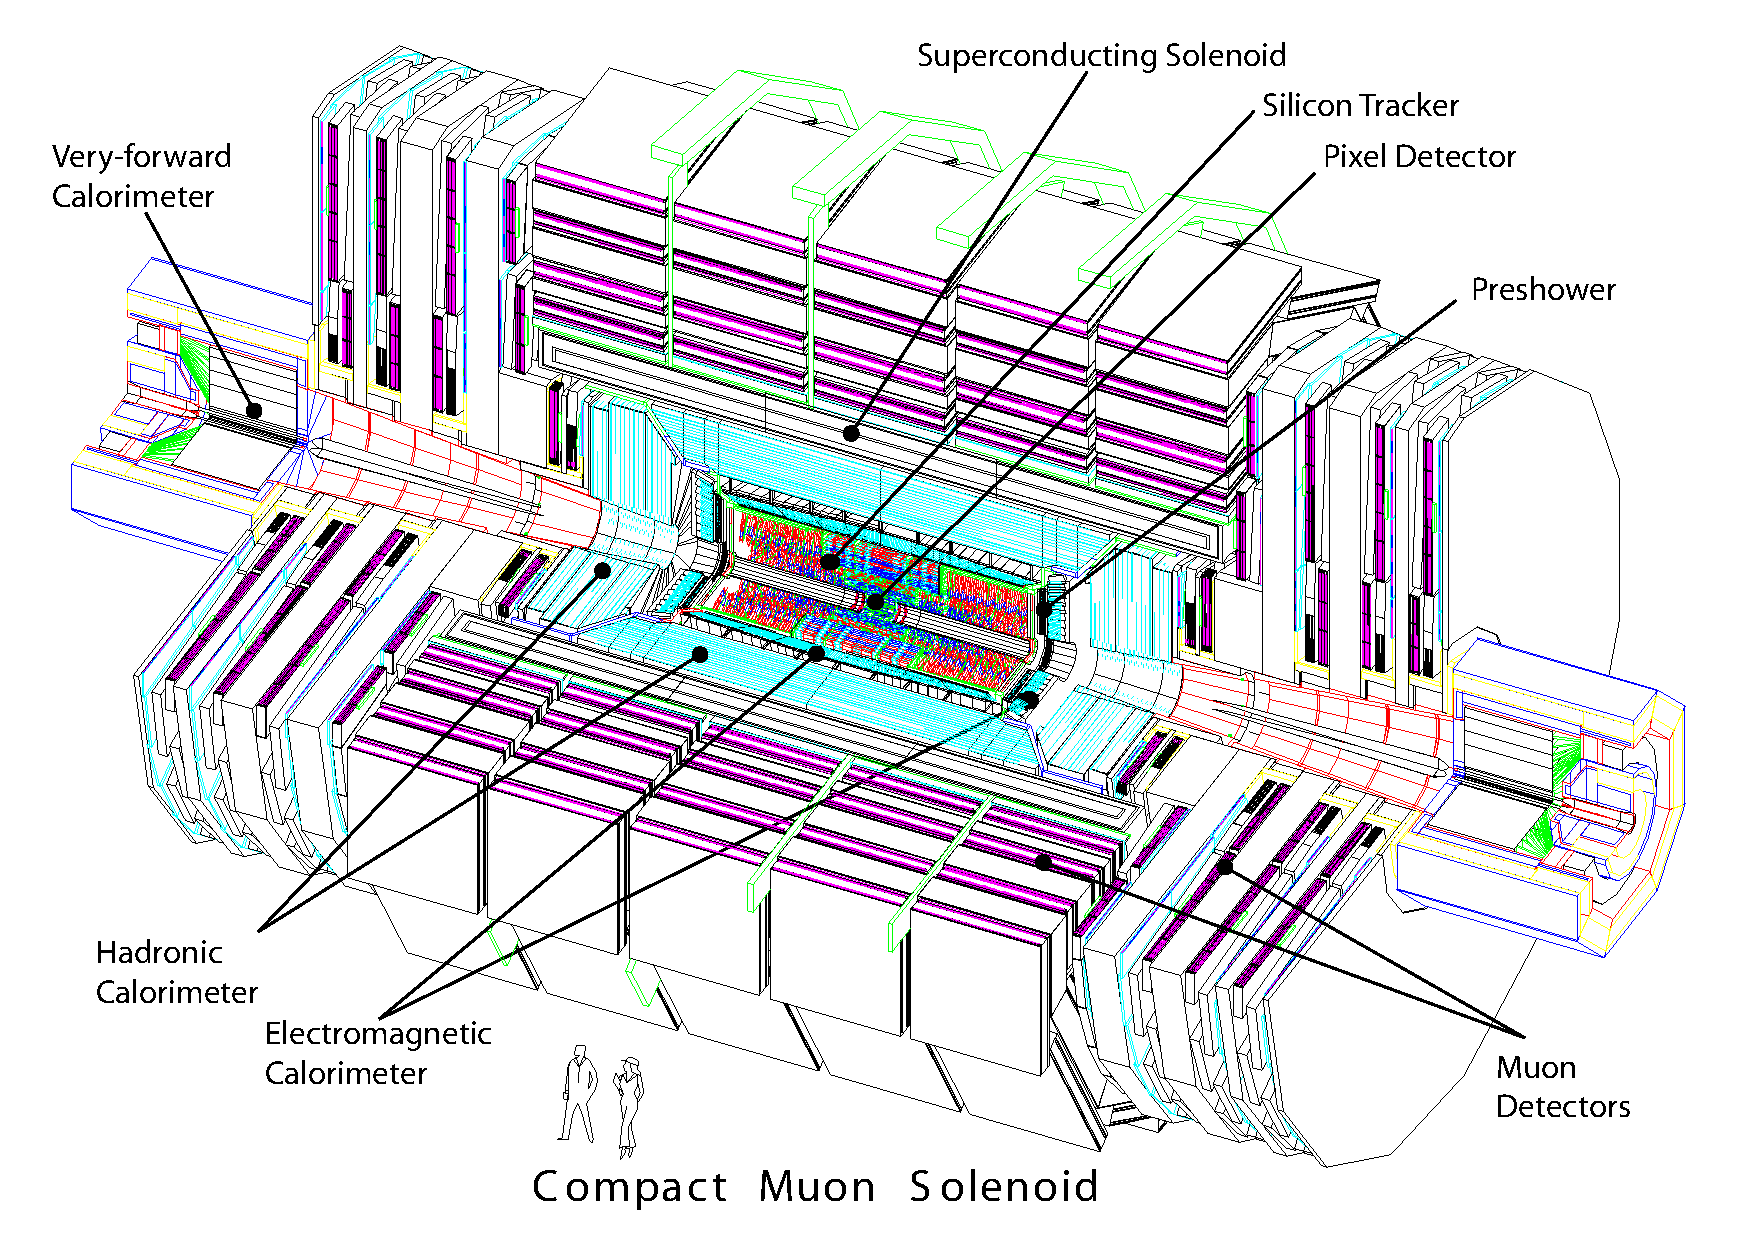
\includegraphics[width=0.7\textwidth]{fig/cms_complete_labelled}
\caption[Illustration of the \acs{CMS} detector]{Illustration of the \ac{CMS}
  detector with subdetectors labelled~\cite{cms_jinst}.}
\label{fig:expt_cms}
\end{figure}

\ac{CMS} adopts a traditional cylindrical design (see
\fig~\ref{fig:expt_cms}), \unit{21.5}{\metre} in length and \unit{15}{\metre}
in diameter. A key feature of the detector is the \unit{4}{\tesla}
superconducting solenoid. The bending field supplied provides accurate muon
momentum resolution up to energies of \unit{$\approx$ 1}{\TeV}. The size of the
solenoid placed stringent limitations on the volume of the inner detector
subsystems (everything except for the muon chambers and return yoke).

\subsection{Coordinate System}
The coordinate system at \ac{CMS} is right-handed, with its origin placed at the
nominal beam collision point inside \ac{CMS}. The $x$ axis is then defined to
point horizontally inwards towards the centre of the \ac{LHC} ring and the
$y$-axis, vertically upwards. The $z$-axis is aligned along the beam-line,
pointing towards the nearby Jura mountains. Often a cylindrical coordinate
system will be used where the azimuthal angle, $\phi$, and radial
coordinate, $r$, span the $x-y$ plane. The azimuthal angle is measured with
respect to the $x$-axis. The pseudorapidity, $\eta = - \ln \tan
\frac{\theta}{2}$ where $\theta$ is the polar angle measured with respect to the
$z$-axis.

\subsection{Silicon Tracker}
The innermost subsystem of \ac{CMS} is the silicon tracker~\cite{tracker_paper},
designed to provide highly precise measurements of particle trajectories close
to the CMS interaction point. It is shown in cross section in
\fig~\ref{fig:expt_tracker}. The tracker extends to pseudorapidities of
$|\eta|<2.5$ and has an active silicon area of more than
\unit{200}{\metre\squared}, making it the largest silicon tracker ever built.

\begin{figure}[h!]
\includegraphics[width=\textwidth]{fig/tracker2}
\caption[Schematic cross section through the CMS tracker]{Schematic cross
  section through the CMS tracker. Each line represents a detector
  module. Double lines indicate back-to-back modules which deliver stereo
  hits~\cite{cms_jinst}.}
\label{fig:expt_tracker}
\end{figure}

The tracker design can be better understood by considering the expected particle
flux at design luminosity as a function of radial distance, $r$, from the
beam-line.
\begin{itemize}
\item At $ r \approx \unit{10}{\cm}$ the particle flux is highest. Accordingly,
  the innermost layer of the CMS tracker is comprised of hybrid pixels. With an
  area of \unit{$100\times 150$}{\micro\metre\squared}, particle densities are
  $O(10^{-4})$ per pixel per LHC bunch crossing.
\item At a radius \unit{$20 < r < 55$}{\centi\metre}, reduced particle flux allows
  the use of silicon microstrip sensors. With a much larger area of
  $\unit{10}{\centi\metre}\times\unit{80}{\micro\metre}$, average particle
  densities are $O(10^{-2})$ per strip per bunch crossing.
\item At $ r > \unit{55}{\cm}$, still larger silicon strips can be used, with
  sizes up to $\unit{25}{\cm}\times\unit{180}{\micro\metre}$. This gives a
  particle density of $O(10^{-2})$ per strip per bunch crossing.
\end{itemize}

\subsubsection{Pixel Tracker}
The hybrid pixels are placed closest to the interaction point. As well as
maintaining an acceptable particle density per sensor, their close proximity to
the interaction point allows the origin of collision products to be accurately
determined. In the barrel region, 3 layers are placed at mean radii of 4.4, 7.3
and \unit{10.2}{\cm}. The detector has a length of \unit{53}{\cm} in the $z$
direction. The end discs are instrumented with only two layers and are located
at $|z|=34.5, \unit{46.5}{\cm}$. The pixel modules in these layers are arranged
in a ``turbine-like'' layout.

\subsubsection{Strip Tracker}
Further from the interaction point, the tracker is instrumented with silicon
strip detectors. The barrel component can be further divided into the \ac{TIB}
and the \ac{TOB}. The \ac{TIB} is composed of 4 layers and the \ac{TOB} a
further 6. The \ac{TOB} extends to $z = \pm \unit{118}{\centi\metre}$. Beyond
this are the endcaps which can again be split into two components: the \ac{TEC}
made up of 9 disks and the \ac{TID}, 3. The silicon micro-strip sensors are
\unit{320}{\micro\metre} thick and oriented parallel to the $z$-axis in the
barrel and radially in the disks.

Both the \ac{TIB} and \ac{TID} supply up to four measurements in $r\phi$. The
inner two layers of the \ac{TIB} have a strip-pitch of \unit{80}{\micro\metre},
and the outer two, \unit{120}{\micro\metre}. These achieve single point
resolutions of \unit{23 and 35}{\micro\metre} respectively. In the \ac{TID}, the
strip pitch varies between \unit{100 and 141}{\micro\metre}.

The \ac{TOB} uses \unit{500}{\micro\metre} thick sensors with a strip-pitch of
\unit{183}{\micro\metre} in the first four layers and \unit{122}{\micro\metre} in
the outer two. This gives a single point resolution of \unit{53}{\micro\metre}
and \unit{35}{\micro\metre} respectively.

The first two layers of the \ac{TIB}, \ac{TOB} and \ac{TID} and rings 1, 2 and 5
of the \ac{TEC} are so-called ``stereo modules''. These are double-sided modules
where the two layers of strips have a stereo angle of \unit{100}{\milli\radian}
between them. This provides additional resolution in the $z$ measurement in the
barrel (or $r$ in the endcaps). The resolution of this measurement is
\unit{230}{\micro\metre} and \unit{530}{\micro\metre} in the \ac{TIB} and
\ac{TOB} respectively.

\subsection{\acl{ECAL}}
The \ac{ECAL} surrounds the silicon tracker and provides a high resolution
measurement of electromagnetic showers within a homogeneous, hermetic
calorimeter~\cite{ecal_paper}. The barrel region alone comprises 61,200 lead
tungstate (PbWO$_4$) crystals, with 7,324 in each of the two endcaps. This
material was chosen for its high density, short radiation length and small
Moli\`{e}re radius. Scintillation photons are then recorded by \acp{APD} in the
barrel and \acp{VPT} in the endcap. The driving motivation for the \ac{ECAL}
design was the detection of the low-mass favoured Higgs decay channel
$\PH\longrightarrow\gamma\gamma$.

\subsubsection{\acl{EB}}
The \ac{EB} extends in rapidity to $|\eta|<1.479|$ with a crystal segmentation
of $360\times 85$ in $\eta-\phi$ for each half-barrel. Each crystal is slightly
tapered, with a cross-section of $0.0174\times0.0174$ in $\eta-\phi$. The
crystals have a front cross section of \unit{$22\times
  22$}{\milli\metre\squared} and a length of \unit{230}{\milli\metre}
(corresponding to 25.8 radiation lengths).

\subsubsection{\acl{EE}}
The \ac{EE} occupies the rapidity range $1.479 < |\eta| < 3.0$. Crystals are
grouped into $5\times 5$ ``supercrystals'' within a carbon-fibre alveolar
structure. The endcaps are split into two halves, known as ``Dees'', each
holding 3,662 crystals.

The scintillation of the \ac{ECAL} crystals as well as the amplification of the
\acp{APD} varies as a function of temperature. This variation was found to be
\unit{$\approx 4\%$}{\per\celsius}. For this reason, the \ac{ECAL} temperature
is precisely regulated to within \unit{$\pm$ 0.05}{\celsius}.

\subsubsection{\ac{ECAL} Transparency and the \ac{CMS} Laser Monitoring System}
\label{sec:expt_laser_monitoring}
The PbWO$_4$ crystals that make up the \ac{ECAL} are radiation resistant but
quickly suffer a decrease in their optical transmission under
irradiation~\cite{ecal_transparency}. This is a result of the formation of
colour centres which absorb a fraction of the incident light. At a working
temperature of \unit{18}{\celsius}, the damage anneals leading to an equilibrium
in the optical transmission properties -- constant with dose rate. The
consequence of this is a cyclic change in the optical transmission rate of the
crystals as the \ac{LHC} moves between colliding beams and machine
refills. Since this depends on dose rate, the effect is a function of \ac{LHC}
luminosity and rapidity. It is expected to range from a shift of $\sim 2\%$ in
the barrel at low luminosity to $> 10\%$ in the endcaps at high luminosity. The
magnitude of this effect on energy and momentum measurements would be disastrous
if not properly accounted for. Correction for this effect necessitates constant
monitoring of the transparency -- a task performed by the laser monitoring
subsystem~\cite{laser_monitoring}.

Three lasers are used for the transparency measurement: two blue ($\lambda
\approx \unit{440}{\nano\metre}$) and one near-infrared ($\lambda \approx
\unit{796}{\nano\metre}$). The blue laser (with a second fitted for redundancy
purposes) is close to the scintillation emission peak and thus can be used to
track the changes in the crystal transparency. The near-infrared laser is far
from the emission peak and thus relatively stable to changes in the
transparency. This can be used to verify the stability of the system. The lasers
are distributed to the crystals via optical fibres and a series of
fan-outs. Approximately 1\% of the \ac{LHC} beam gap of
\unit{3.17}{\micro\second} is used for transparency monitoring. A full scan of
the entire \ac{ECAL} can be achieved in approximately 30~minutes. The lasers can
be pulsed at $\approx \unit{80}{\mega\hertz}$ with a pulse timing jitter of
\unit{3}{\nano\second}. This is adequate for synchronisation with the \ac{LHC}
bunch crossings.

The transparency of the crystals is derived from the response of the \ac{APD}
normalised to the height of the laser pulse, as measured using a silicon
photodiode. Due to differences in path length and optical spectra between the
laser and the scintillation light, the transparency of the crystals may be
related to the measured transparency via a power law.

\subsection{\acl{HCAL}}
Accurate measurement of hadronic showers is crucial for analyses involving jets
or missing energy signatures. The \ac{HCAL}~\cite{hcal_paper} lies between the
outer edge of the ECAL and the inner edge of the solenoid ($\unit{1.77}{\metre}
< r < \unit{2.95}{\metre}$). This constrains the size of the \ac{HCAL} to a
relatively compact design and necessitates the placement of a ``tail catcher''
outside of the solenoid.

\subsubsection{\acl{HB}}
The \ac{HB} comprises 36 azimuthal wedges, with 18 in each half barrel. Each
wedge consists of alternating layers of brass absorber plates and plastic
scintillators. The light from these plates is then carried via
wavelength-shifting fibres to a \ac{HPD} for readout. The number of interaction
lengths increases with polar angle, from 5.82 at $90\degrees$ to 10.6 at
$|\eta|=1.3$~\cite{hcal_design}.

\subsubsection{\acl{HE}}
The \ac{HE} covers the rapidity range $1.3 < |\eta| < 3$ and receives a larger
radiation flux than the \ac{HB}. Each endcap consists of 36 wedges, and
wavelength shifting fibres are once again used to take light from plastic
scintillators to \acp{HPD}. Including the \ac{ECAL}, the \ac{HE} depth is
equivalent to $\approx 10$ interaction lengths.

\subsubsection{\acl{HO}}
The \ac{HO} or ``tail catcher'' provides increased sampling depth in the
rapidity region $|\eta| < 1.3$ where the \ac{HB} and \ac{EB} do not provide
sufficient containment. Since the \ac{HO} lies outside the solenoid, its design
is constrained by that of the muon chambers -- with 5 rings in $\eta$. The
solenoid coil provides additional absorption, giving the calorimeter system a
minimum depth of 11.6 interaction lengths.

\subsubsection{\acl{HF}}
The \ac{HF} is positioned in the rapidity range $|\eta|>3$ and consequently must
endure a much larger particle flux -- approximately \unit{760}{\GeV} per
proton-proton interaction (versus $\approx \unit{100}{\GeV}$ for the rest of the
detector). Radiation hardness was thus a leading consideration in its design.

Quartz fibres are interleaved between steel absorbers. Shower particles above
the Cherenkov threshold ($E \geq \unit{190}{\keV}$ for electrons) produce
Cherenkov light. This is routed to the rear of the calorimeter and read out by
\acp{PMT}. The \ac{HF} is most sensitive to the electromagnetic component of the
shower.

\subsection{Muon Chambers}
Accurate measurement of muons is one of \ac{CMS}' key design goals. The effect
of radiative losses in the tracker is much less for muons than it is for
electrons. Thus muons are able to provide a much finer mass resolution at low
transverse momentum. This is an important advantage for a variety of physics
searches and measurements at \ac{CMS}. The muon system is responsible for muon
identification, momentum measurement and triggering (for further detail see
\sec~\ref{sec:trigger}). Three types of detectors are used, chosen for different
regions of the detector according to the magnetic field, muon rate and response
time required for input to the trigger.

\subsubsection{\aclp{DT}}
In the barrel region, the magnetic field is relatively uniform and the muon flux
low enough to allow the use of the \acf{DT}~\cite{dt_paper}. These identify
muons in the region $|\eta| < 1.2$. The drift chamber was first developed as a
refinement of earlier wire proportional chamber designs in which the drift time
of the electrons to the anode wire is used to provide additional spatial
resolution. This allows the wire spacing to be increased, thus reducing the
electronics requirements.

Each \ac{DT} is composed of 2 (or 3) ``super-layers'', with each super-layer
further divided into 4 layers of rectangular drift cells. Of the four concentric
muon stations in the barrel, the inner three contain 60 drift chambers and the
outermost, 70. The wires in the outer two layers of each drift cell are oriented
parallel to the beam line, providing a measurement in the $r\phi$ direction (the
magnetic bending plane). The inner two layers are perpendicularly aligned,
giving a measurement of the $z$ coordinate.

\subsubsection{\aclp{CSC}}
In the endcap region, the large muon and background rate coupled with the
strong, non-uniform magnetic field, prevent the use of \acp{DT}. Instead, an
alternative instrument is used -- the \ac{CSC}~\cite{csc_paper}. The CMS muon
system endcap consists of 468 \acp{CSC}, each a trapezoidal multiwire
proportional chamber arranged radially covering an azimuthal angle $\Delta\phi$
of either 10 or 20 degrees. Each \ac{CSC} has 6 anode wire planes interleaved with 7 cathode strip planes. The wire
readout provides a measurement of the $r$ coordinate whilst a measurement of
$\phi$ is obtained by interpolating charges on the cathode strips.

\subsubsection{\aclp{RPC}}
The trigger (see \sec~\ref{sec:trigger}) requires a muon detector capable of
providing a fast signal with adequate spatial resolution. This is the
\acf{RPC}~\cite{rpc_paper}, a gaseous, parallel-plate detector with spatial
resolution suitable for both barrel and endcap regions and a response time much
less than the \unit{25}{\nano\second} between consecutive \ac{LHC}
bunch-crossings. This allows the \ac{RPC} to unambiguously identify the
bunch-crossing assignment for a muon track, even in the presence of the large
backgrounds and high rates of the \ac{LHC} environment.

\subsection{Data Acquisition and Trigger System}
\label{sec:trigger}
The high luminosity of the \ac{LHC} beam leads to a high particle flux in the
detector. The separation of particles in the detector becomes increasingly
difficult. In addition, many analyses benefit from precise position and momentum
measurements. Consequently, the \ac{CMS} subdetectors are constructed with an
extremely fine granularity. Unavoidably, this requires an extremely large number
of read-out channels - approximately 55 million across the whole detector. To
make matters worse, the \ac{LHC} is planned to achieve a bunch-spacing of only
\unit{25}{\nano\second}. For these reasons, the \ac{DAQ} system at \ac{CMS}
faces the simultaneous challenges of large bandwidth and low-latency.

Tightly coupled to the \ac{DAQ} is the trigger system~\cite{tridas}. The huge
number of readout channels in \ac{CMS} is not only a challenge in terms of the
bandwidth of the \ac{DAQ} but also poses serious difficulties relating to
long-term storage requirements. A digitised, zero-suppressed event dump from
\ac{CMS} is approximately \unit{2}{\mega\byte} in size. With an event rate of up
to \unit{40}{\mega\hertz}, this would require a storage rate of
\unit{80}{\tera\byte\per\second}. Despite the rapid improvement in disk storage
technology over the last few decades, such storage capacities are clearly
infeasible both in terms of capacity and \ac{IO} requirements. For these
reasons, a system capable of quickly rejecting a very large fraction of
collisions is required. This is known as the trigger.

\subsubsection{Triggering at \ac{CMS}}
The trigger at \ac{CMS} is split into two stages. The first stage, the \ac{L1T},
must operate at the full \ac{LHC} bunch-crossing frequency. To achieve adequate
latency, it is implemented almost entirely within electronic logic -- either
\acp{FPGA} or custom designed integrated circuits. The \ac{L1T} must reduce the
rate to \unit{100}{\kilo\hertz}.

In the second stage of the trigger, the \ac{HLT}, the rate is further reduced to
$O(\unit{100}{\hertz})$. Due to the reduced rate, the \ac{HLT} is implemented in
software running in a computing farm. Since the \ac{HLT} has access to a full
read-out of the detector, and more time to issue a trigger decision, more
sophisticated trigger algorithms are used. Often these are similar to those used
by the off-line reconstruction.

\subsubsection{The \acl{L1T}}
The \ac{L1T} must produce a trigger decision with minimal latency. This latency
is chiefly limited by the size of the pipeline on the \ac{APV25} chip used to
readout from the silicon strip tracker. The \ac{APV25} samples the voltage from
the silicon strips at \unit{25}{\nano\second} intervals. These are stored in a
pipeline, 192 samples deep. This constrains the \ac{L1T} to provide a decision
within $\approx \unit{3.2}{\micro\second}$.

The \ac{L1T} has limited access to detector subsystems and only a limited time
in which to issue a trigger decision. In particular, since tracker measurements
are not available, distinction between electrons and photons is not
possible. The challenge for the \ac{L1T} is therefore not only to make a fast
decision using limited information from the detector, but also to ensure that
potentially interesting events are retained and passed onto the \ac{HLT} for
more thorough analysis.

\begin{figure}[h!]
\centering
\includegraphics[width=0.7\textwidth]{fig/trigger}
\caption[Diagram showing the organisation of the \acs{CMS} \acs{L1T}]{Diagram
  showing the organisation of subsystems within the \ac{CMS} \ac{L1T}.}
\label{fig:expt_cms_trigger}
\end{figure}

The structure of the \ac{L1T} is shown in \fig~\ref{fig:expt_cms_trigger}. The
\ac{GT} is the final stage in the trigger chain. It receives ``trigger objects''
from two subsystems: the \ac{GCT} and \ac{GMT}. Objects, ranked according to
their energy and quality, are received along with their coordinates in $\eta$
and $\phi$. These objects are processed by 128 algorithms, each of which
produces a trigger decision. The final output of the \ac{GT} is then determined
by a configurable mask, which may be altered to meet different data-taking
objectives. The final trigger decision is then sent to the Timing, Trigger and
Control subsystem in order to initiate a read-out of the detector.

The calorimeter trigger subsystem begins with the \ac{TPG}. This sums energy
deposits from the \ac{ECAL} and \ac{HCAL} into ``trigger towers''. These are
received by the \ac{RCT}, where electron/photon candidates are found and the
trigger tower energies summed into larger ``\ac{RCT} regions''. These consist
of $4\times 4$ trigger towers (except in the \ac{HF} where only a single trigger
tower is included). The \ac{RCT} also records a ``tau-veto'' bit, used to
distinguish jets from hadronic tau decays.

The output of the \ac{RCT} is then processed by the
\ac{GCT}~\cite{jj_thesis}. The \ac{GCT} logic is implemented primarily in
\acp{FPGA}. The \ac{GCT} performs a number of tasks in parallel. It sorts the
list of electron/photon candidates and passes the four highest ranked objects to
the \ac{GT}. It also performs a simple jet-finding algorithm on the \ac{RCT}
regions, classifying them as \emph{forward}, \emph{central} and \emph{tau}
jets. The last category includes jets for which none of the constituent \ac{RCT}
regions has its tau-veto bit set. The four highest ranked of each category are
then forwarded to the \ac{GT}.

The final task of the \ac{GCT} is to form global energy sums. These are the
total transverse energy, missing transverse energy, jet counts and \HT (the
scalar sum of the jet energies). These too are forwarded to the \ac{GT}.

The muon trigger receives input from all three muon subdetectors: \acp{RPC},
\acp{CSC} and \acp{DT}. These are integrated in the \ac{GMT}. The muons received
from each subdetector are matched and sorted by transverse momentum and
quality. The four highest rank candidates are forwarded to the \ac{GT}.

\subsection{Computing at \acs{CMS}}
\label{sec:cms_computing}
To meet the extremely large computation and storage requirements of data analysis
at the \ac{LHC}, analysis tasks are performed using a dedicated computing
grid~\cite{lhc_grid}. Events are first sent to the ``tier-0'' storage site at
\ac{CERN} with additional copies forwarded to a number of ``tier-1'' sites
around the world. Data is made available for analysis use, in various
re-processed forms, at ``tier-2'' and ``tier-3'' grid sites. User analysis jobs
are submitted to the grid, and routed automatically to a suitable site.

Events recorded by the \ac{CMS} detector pass through a chain of reconstruction
stages. At each stage, higher-level physics objects are built out of simpler
ones, with a consequent reduction in the data size. \ac{MC} events are processed
using either a detailed \geantfour simulation~\cite{geant_paper}, or a faster,
parameterised model of the response known as \fastsim. This simulates the
response of the \ac{CMS} subdetectors to the generated particles. After the
detector response has been simulated, \ac{MC} is processed in exactly the same
manner as data.

  \chapter{Physics Objects}
\section{Introduction}
In the previous chapter, details of the \ac{CMS} detector were presented. We
shall now begin to discuss the reconstruction algorithms used to derive analysis
level objects and quantities which will be of fundamental importance in later
chapters. The objects of primary interest for these purposes are the leptons,
jets and missing energy. The offline reconstruction algorithms used to
reconstruct each object will be presented, along with issues and properties
related to data analysis. Some details of the reconstruction performance at
\ac{CMS} will also be shown. Finally, the \acl{PF} method, which provides a
global reconstruction of the event, will be explained in some detail. As will be
seen, \ac{PF} combines tracking and calorimeter measurements to provide
excellent reconstruction of jets and missing energy.

\section{Leptons}
\subsection{Muons}
The full details of muon reconstruction at CMS are presented in
\cite{cms_mu_reco}, \cite{cms_mu_pas}. A brief overview will be presented here, focussing on the
aspects pertinent to the following analysis chapters. Muons are reconstructed in
both the muon chambers and the silicon tracker. To match this redundancy in the
measurement, a number of reconstruction algorithms are available.

\subsubsection{Global Muons}
Global muons are an extension of standalone muons to include measurements in the
silicon tracker. For muons with a transverse momentum below $\approx$
\unit{200}{\GeV}, the tracker provides a better momentum resolution. For higher
momentum muons, the tracks become straighter and the momentum measurement
increasingly affected by uncertainty in the position measurement. In this
regime, inclusion of hits in the muon chambers effectively benefits from the
large lever arm and \unit{3.8}{\tesla} magnetic field in the region between the
silicon tracker and the muon chambers.

For each standalone muon, the set of tracker tracks is searched and the best
matching candidate selected. For each pairing found in this way, a Kalman-filter
fit is again performed, this time using hits from both the silicon tracker and
the muon chambers. This fit accounts for average expected energy losess,
magnetic field and multiple scattering effects. The tracks reconstructed by this
procedure are known as global muons. Once again, certain modofications are
required for reconstructing cosmic ray muons - for instance in the case that
cosmic muons traverse the entire detector, leaving two standalone muons on
either side of \ac{CMS}.

\subsubsection{Tracker Muons}
Tracker muons, in contrast to Global muons begin as tracks in the silicon
tracker. All tracks with a $\Pt > \unit{0.5}{\GeV}$ and $p > \unit{2.5}{\GeV}$
are considered as muon candidates and extrapolated to the muon stations,
accounting for expected energy loss and multiple scattering effects. If at least
one muon track segment matches the extrapolated tracker track, a tracker muon is
reconstructed. This algorithm is more efficient at low momentum ($p <
\unit{5}{\GeV}$) since it requires only a single segment in the muon chambers.

\subsubsection{Standalone Muons}
Standalone muons are based solely on measurements in the muon chambers. The hits
in each chamber are fit individually to obtain seeds - a position and direction
vector along with an estimate of the transverse momentum. These form the basis
of a track fit in the muon chambers based on the Kalman-filter technique. The
fit is constrained to the vertex in order to reject cosmic ray muons. Since much
of the callibration and validation work for the muon system was performed using
cosmic rays, a separate algorithm was developed for this purpose
\cite{cms_mu_reco_cosmic}.

\subsubsection{Merging}
Reconstructed muons from each of the algorithms detailed above are then merged
into a single list of muon candidates. Candidates reconstructed as both global
and tracker muons are merged. Standalone muon tracks are merged with tracker
muons if they share a muon segment. The fit results from each algorithm are
retained.

An analysis is then able to tune its identification cuts to meet certain
efficiency or purity requirements for a particular kinematic range. A selection
of pre-defined selections are available:
\begin{itemize}
\item Soft muons are required to be reconstructed as tracker muons with a muon
  segment in the outermost station matching the position and direction expected
  from extrapolation of the track.
\item Global muon's only requirement is that they be reconstructed as a global
  muon in the sense described above.
\item Tight muons must be reconstructed as both a global muon and a tracker muon
  with a series of additional requirements: a $\Pt > \unit{3}{\GeV}$, a global
  muon track fit with a normalised $\chisq < 10$, at least two muon stations
  with matching muon segments, at least 10 hits in the silicon tracker (with at
  least 1 pixel hit) and a transverse impact parameter $\dxy <
  \unit{2}{\milli\metre}$. This selection significantly supresses
  decays-in-flight at the cost of a small loss in efficiency for prompt muons.
\end{itemize}


\subsection{Electrons}
Electron reconstruction at \ac{CMS} makes use of measurements from both the
silicon tracker and the \ac{ECAL}. In the case of \ac{CMS}, the material budget
of the tracker cause electrons to radiate a large fraction of their energy
before reaching the \ac{ECAL} - 50\% of electrons radiate more than 50\% of
their energy in this way. For an accurate measurement of the electron energy,
this energy, radiated in the form of bremsstrahlung photons, must be
reconstructed correctly.

\subsubsection{Reconstruction}
Electron seeds are derived by two separate algorithms: tracker driven and
\ac{ECAL} driven. Tracker driven seeds are suitable for low-\Pt electrons and
for electrons produced inside jets. \ac{ECAL} driven seeds begin with the
reconstruction of \ac{ECAL} superclusters with transverse energy $\Et >
\unit{4}{\GeV}$. Superclusters are a group of one or more \ac{ECAL} clusters
constructed to account for the width energy spread in $\phi$ and narrow width in
$\eta$ characteristic of the bending effect of the \ac{CMS} magnet on electrons
radiating in the tracker. The supercluster seeds are first matched to track
seeds (2 or 3 hits) in the inner layers of the tracker. Electron tracks are then
built from these track seeds. The trajectory is reconstructed accounting for the
electron energy loss and fitted with a \ac{GSF}.

\subsubsection{Electron Identification}
\label{sec:reco_electron_id}
The large bremsstrahlung induced energy loss coupled with larger backgrounds
from jets and photons means that electrons at \ac{CMS} are fundamentally less
well defined object than muons. There is therefore a much larger space to trade
between signal efficiency and purity. Whilst more complex selection procedures
are available (e.g. a multivariate approach), a simple cut-based selection was
chosen for the \PW cross-section measurement\cite{cms_pas_ewk_10_002} and has been
used in this work. The variables have been chosen for their background rejection
capabilities but also for robustness during early the data-taking period. Cut
values have been chosen for a number of working points, defined by their
efficiency with respect to a simulated \Wenu sample, and optimising the
background rejection power using an iterative procedure. Different cut values
are chosen in the \ac{CMS} barrel and encap regions.

The cut variables used are described below, with cut-values for eaching working point shown in Table~\ref{tbl:reco_electronid}
\begin{itemize}
\item \sigmaieta is a measure of the \ac{RMS} shower width of the electron
  in the $\eta$ direction.
\item \deltaphiin and \deltaetain represent the angular separation between the
  trajectory of the \ac{GSF} track and the ac{ECAL} supercluster.
\item Tracker, \ac{ECAL} and \ac{HCAL} isolation quantities summed in a cone
  $\Delta R < 0.3$. Within the tracker, a threshold of \unit{700}{\GeV} is
  applied to the tracks contributing to the sum. Similarly, in the ac{ECAL}, a
  zero-supression cut is applied. The cone is centred on the track direction at
  the vertex for the tracker isolation, and the supercluster for the calorimeter
  quantities.
\item \HoverE is the ratio of the energy deposited in the \ac{HCAL} behind the
  electron seed to that in the \ac{ECAL}. This might also be called the
  \ac{HCAL} leakage.
\item The track associated with the electron is required to have a hit in the
  first layer of the pixel tracker in order to reject photon conversions.
\item Further rejection against electron conversions is provided by the
  variables \Dist and \DeltaCotTheta. These are calculated by searching for a
  conversion partner of the electron \ac{GSF} track. If such a partner is found,
  the electron is rejected if both \Dist and \DeltaCotTheta are below given thresholds.
\end{itemize}

\ctable[
caption=Simple Cut-Base Electron ID Working Points,
label=tbl:reco_electronid
]{lcccccc}{
}{\FL
Efficiency           & 0.95  & 0.9   & 0.85  & 0.8   & 0.7   & 0.6 \ML
\multicolumn{7}{c}{Conversion Rejection}\ML
Missing Hits         & 1     & 1     & 1     & 0     & 0     & 0 \NN
\Dist                & -     & 0.02  & 0.02  & 0.02  & 0.02  & 0.02\NN
\DeltaCotTheta       & -     & 0.02  & 0.02  & 0.02  & 0.02  & 0.02\ML
\multicolumn{7}{c}{Barrel}\ML
Combined Isolation   & 0.15  & 0.1   & 0.09  & 0.07  & 0.04  & 0.03 \NN
\sigmaieta           & 0.01  & 0.01  & 0.01  & 0.01  & 0.01  & 0.01 \NN
\deltaphiin          & 0.8   & 0.8   & 0.06  & 0.06  & 0.03  & 0.025 \NN
\deltaetain          & 0.007 & 0.007 & 0.006 & 0.004 & 0.004 & 0.004 \NN
\HoverE              & 0.15  & 0.12  & 0.04  & 0.04  & 0.025 & 0.025 \ML
\multicolumn{7}{c}{Endcaps}\ML
Combined Isolation   & 0.1   & 0.07  & 0.06  & 0.06  & 0.03  & 0.02 \NN
\sigmaieta           & 0.03  & 0.03  & 0.03  & 0.03  & 0.03  & 0.03 \NN
\deltaphiin          & 0.7   & 0.7   & 0.04  & 0.03  & 0.02  & 0.02 \NN
\deltaetain          & 0.01  & 0.009 & 0.007 & 0.007 & 0.005 & 0.005 \NN
\HoverE              & 0.07  & 0.05  & 0.025 & 0.025 & 0.025 & 0.025 \LL
}

\subsubsection{\ac{ECAL} Transparency Corrections}
\label{sec:reco_ecal_transparency}
\section{Jets}
Four types of jets are reconstructed at \ac{CMS}: \acp{Calo} jets, \ac{PF} jets,
\ac{JPT} jets and track jets. \ac{Calo} jets are reconstructed from energy
deposits in the \ac{ECAL} and \ac{HCAL}, combined into calorimeter
towers. Calorimeter towers consist of one or more \ac{HCAL} cells with
geometrically matched \ac{ECAL} crystals. The exact details of this association
varies between the barrel and endcap regions. Electronics noise is supressed by
applying a threshold to calorimeter cells, with pile-up effects reduced by a
requirement on the tower energy.

\ac{JPT} jets associate tracks with \ac{Calo} jets, using the tracker to give
enhanced \Pt resolution and response. \ac{PF} jets are products of the \acl{PF}
algorithm described below. Finally, track jets are reconstructed from well
measured tracks in the central tracker.

Jets are clustered using the \antiKT algorithm \cite{antiKT} with a size
parameter $R=0.5$.

\section{Missing Energy}
A missing energy measurement is made by considering the total momentum of some
set of particles reconstructed in the detector and comparing this quantity to
the initial momenta of the colliding partons. Any difference in these two
quantities may be attributed to the presence of additional particles, not
interacting within the volume of the detector. There are a number of ways to
define such a signal. At a hadron collider, the initial boost of the parton
along the beam axis is unknown. For this reason, the transverse component of the
missing energy is normally taken instead.

Missing transverse energy (\MET) is the most commonly used missing energy
quantity. \MET can be measured in several ways at \ac{CMS}. Most simply, via
\ac{Calo} \MET, which takes the negative vector sum of calorimeter tower
energies (\ac{ECAL} and \ac{HCAL}). An energy threshold is applied to the towers
contributing to the sum to reject electronics noise. Alternatively, \ac{PF} \MET
instead takes the negative vector sum over the momenta of particles
reconstructed according to the \acl{PF} algorithm. As can be seen in Section~
\ref{sec:reco_pf}, this has been shown to provide the most sensitive \MET
measurement at \ac{CMS}. Unless explicitly noted, it should be assumed that all
\MET quantities in this work are calculated in this way.

Alternative missing energy quantities can be defined for other purposes. For
instance, missing transverse hadronic energy (\MHT) is formed by taking the
vector sum,
\begin{equation}
\MHT = -\sum_{j \in \textrm{jets}} \vec{E_T^j}
\end{equation}
This gives the energy of a system recoiling against jets in the event. For
instance, in a \Wjets event, the lepton and neutrino recoil against the jets in
the event. The \MHT is therefore a measure of the \PW momentum.


\section{Particle Flow at \ac{CMS}}
The \ac{PF} algorithm \cite{cms_pf_pas} attempts to provide a global
reconstruction of the event - accurate determination of the type, energy and
direction of all stable particles - by combining measurements from all
subdetectors in \ac{CMS}. This strategy is well suited for use with the \ac{CMS}
detector. The silicon tracker is able to reconstruct charged particle tracks
with high efficiency and low fake rate down to transverse momenta as low as
\unit{150}{\MeV}. Additionally, the granularity of the \ac{ECAL} is sufficient
for the separation of photons and charged particle energy deposits in jets with
\Pt of a few hundred \GeV. In contrast, the \ac{HCAL} is much coarser. However,
the combined energy resolution of both calorimeters is $\sim 10\%$ at
\unit{100}{\GeV}. This allows identification of the energy deposits associated
with neutral hadrons as an excess on top of that accounted for by matching the
deposits with charged tracks. The \ac{PF} algorithm is able to reconstruct the
components of jets and hadronic tau decays - primarily charged hadrons, neutral
hadrons and photons. This provides an improved measurement of the jet energy and
thus also of \MET.

The particle flow algorithm procedes by linking the tracks and energy clusters
to form blocks. A single block main contain some combination of a charged
particle track, one or more energy clusters and a muon. The fine granularity of
the \ac{CMS} detector ensures that blocks typically contain 1, 2 or 3 elements.
The links between each block are parameterised by a distance which encodes the
quality of the link. In order for \ac{PF} reconstruction to work correctly, it
is important that the inputs to the algorithm match certain requirements

\subsection{Iterative Tracking}
The measurements of momentum and direction of charged hadrons provided by the
tracker are hugely superior to those that can be provided by the calorimeters.
It is important therefore that the tracks input to the \ac{PF} procedure be
reconstructed with near 100\% efficiency. The fake rate must also be low to
avoid excess energy counting.

To meet these requirements, tracks are reconstructed using an iterative
algorithm. This begins by reconstructing tracks with very tight selection
requirements. Hits which can be unambiguously assigned in this step are then
removed from consideration and the remaining hits are reconstructed again, this
time with loosened selection criteria. This procedure is repeated with
progressively looser selection criteria ensuring high efficiency, whilst the
removal of hits at each stage reduces the fake rate induced by combinatorics.
After three iterations, tracks originating close to the beam line are
reconstructed with an efficiency of 99.5\% for muons and $>90\%$ for charged
hadrons. The fourth and fifth iterations relax constrains on the vertex,
reconstructing secondary charged particles.

\subsection{Calorimeter Clustering}
The success of the \ac{PF} reconstruction is dependent on certain aspects of the
clustering algorithm. In particular, as for the tracks, the clustering needs to
be highly efficient and be able to distinguish closely spaced energy deposits.
To this end, a specialised clustering algorithm was developed. This algorithm is
used the \ac{ECAL}, \ac{HCAL}, \ac{PS} but not in the \ac{HF} where each cell is
taken to be a cluster.

The first step of the algorithm produces seed clusters from local maxima in the
calorimeter cells above a given energy. The second step produces topological
clusters by extending cluster two include cells with at least one side in common
with the cluster and an energy above a threshold related to the standard
deviation of the electronics noise in the calorimeter. The topological clusters
are then transformed to particle flow clusters, with a separate particle flow
cluster for each seed comprising the topological cluster. The energy and
position of each particle flow cluster is determined iteratively with the energy
of each seed shared between the particle flow clusters.

\subsection{Building Links}
Each track is extrapolated from the position of its last measured hit to the
\ac{PS}, the \ac{ECAL} at a depth corresponding to the expected maximum for an
electron shower, the \ac{HCAL} at a depth of 1 interaction length. If the
extrapolated track position lies within the envelope of a cluster, a link is
created with a link distance equal to the $(\eta, \phi)$ distance between the
extrapolated track and the cluster. The envelope may be enlarged with respect to
the cluster by the extent of a single cell.

Additionally, energy contributions from bremsstrahlung photons are included by
extrapolating the track tangent at each tracker layer to the \ac{ECAL}. If the
extrapolated track lies within the envelope of the cluster, a link is created.
Links are also created between calorimeter clusters in different subdetectors if
the cluster position in the finer-grained calorimeter lies within the envelope
of the more coarsely grained calorimeter. The link distance is taken to be the
$(\eta, \phi)$ separation of the two clusters.

Muons are included when a global fit between a track in the tracker and a muon
track in the muon chambers yields an acceptable \chisq. If several global muons
are found for a single muon track, only that possessing the smallest \chisq is
retained - with the link distance determined by the \chisq.

\subsection{Particle Reconstruction}
The first step is to reconstruct muons. Each global muon gives rise to a
particle flow muon providing its momentum as determined from the global fit is
compatible with the track momentum to within 3 standard deviations. The
corresponding track is then removed from the block.

The next step is electron reconstruction. Electron tracks in the block are first
selected by a pre-identification step - electrons often leave short tracks and
lose energy via bremsstrahlung. Pre-identified electrons are then refit with a
Gaussian Sum Filter (see Section~TODO) and projected into the \ac{ECAL}.
Candidates passing tracking and calometric criteria are reconstructed as
particle flow electrons. The track and associated \ac{ECAL} clusters are then
removed from the block.

Tracks remaining are then subject to a tighter set of quality requirements, in
particular that the track \Pt uncertainty be smaller than the relative
calorimeter energy resolution for a charged hadron. Whilst some real hadrons are
lost by this requirement, the energy will be retained in the more accurate
measurement of the calorimeter.

Reconstruction of photons and neutral hadrons involves comparison of the track
momentum to the calorimetric energy. The cluster energies in the \ac{ECAL} are
callibrated for photons and the \ac{HCAL} for \unit{50}{\GeV} pions. For the
comparison to be valid, these must be recallibrated to account for
non-linearities in the \ac{HCAL} as well as the differing response of the
\ac{ECAL} to hadrons.

In the case that several tracks are linked to a single \ac{HCAL} cluster, the
total momenta of the tracks is compared to the callibrated calorimetric energy.
Tracks linked to multiple clusters are resolved by preserving the closest link
or links in certain cases. The track momentum is then compared to the total
callibrated calometric energy.

In the rare case that the energy is smaller than the track momentum by more than
three standard deviations, a relaxed search for fake tracks and global muons is
initiated. Global muons are identified as \ac{PF} muons if their momentum is
measured with an uncertainty below 25\%. Tracks are then progrssively removed
from the block, those with largest momentum uncertainty first, until either all
tracks with an uncertainty $>\unit{1}{\GeV}$ have been considered or the total
track momentum has decreased below the calorimetric energy. The reamining tracks
are interpreted as charged hadrons with momentum and energy taken from the track
momentum assuming the charged pion mass hypothesis. If the calorimeter energy
and track momentum are compatible within their uncertainties, the momentum is
redefined by a fit to both track momenta and the energy cluster. This is helpful
at very high energies, where the track parameters may be less well measured.

In the case that the callibrated energy is greater than the total track momentum
by more than the caloririmetric energy resolution, the excess is interpreted as
a photon and possibly a neutral hadron. If the excess is greater than the
\ac{ECAL} energy, a photon is created with this energy and the rest of the
excess interpreted as a neutral hadron. Otherwise, a photon only is
reconstructed from the uncallibrated \ac{ECAL} energy. This stems from the
observation that photons carry 25\% of the energy of a jet, with neutral hadrons
only 3\%.

Remaining \ac{ECAL} and \ac{HCAL} clusters not linked to a track (or for which
the associated track was disabled in the previous steps) are reconstructed as
photons and neutral hadrons respectively.

So called \ac{PF} jets are then reconstructed using a traditional jet clustering
algorithm (see Section~TODO) using the full set of particle flow objects.

\subsection{Physics Performance}
Two aspects of the performance of the \ac{PF} reconstruction are of relevance to
the analysis description that will follow: \acl{MET} measurement and jet
reconstruction.


\begin{figure}
\centering
\subfloat[]{\label{fig:reco_pf_jet_energyres_barrel}\includegraphics[width=0.45\textwidth]{fig/pf_jet_energyres_barrel}}\quad
\subfloat[]{\label{fig:reco_pf_jet_energyres_endcap}\includegraphics[width=0.45\textwidth]{fig/pf_jet_energyres_endcap}}\quad
\caption[]{Jet energy resolution as a function of \Pt for the
  \subref{fig:reco_pf_jet_energyres_barrel} barrel and
  \subref{fig:reco_pf_jet_energyres_endcap} endcap. Calo-jet values are
  displayed as open squares and \ac{PF} jet as upwards triangles. The curves are
  fit to the sum of a constant term, a stochastic term and a noise term.}
\label{fig:reco_pf_jet_energyres}
\end{figure}

\begin{figure}
\centering
\subfloat[]{\label{fig:reco_pf_jet_etares}\includegraphics[width=0.45\textwidth]{fig/pf_jet_etares}}\quad
\subfloat[]{\label{fig:reco_pf_jet_phires}\includegraphics[width=0.45\textwidth]{fig/pf_jet_phires}}\quad
\caption[]{Jet angular resolution (\ac{RMS}) as a function of \Pt for
  \subref{fig:reco_pf_jet_etares} $\eta$ and \subref{fig:reco_pf_jet_phires}
  $\phi$. Calo-jets are shown as open squares and \ac{PF} jets as upward
  triangles. The curves are fit with an expontential function of $\Pt$.}
\label{fig:reco_pf_jet_angulares}
\end{figure}

\begin{figure}
\centering
\subfloat[]{\label{fig:reco_pf_met_metres}\includegraphics[width=0.45\textwidth]{fig/pf_met_metres}}\quad
\subfloat[]{\label{fig:reco_pf_met_phires}\includegraphics[width=0.45\textwidth]{fig/pf_met_phires}}\quad
\caption[]{\subref{fig:reco_pf_met_metres}$\sigma(\MET)/\MET^{\textrm{true}}$ and
  \subref{fig:reco_pf_met_phires} $\sigma(\phi)$ as a function of true \MET in
  \ttbar events as detmined by a Gaussian fit to each $\MET^{\textrm{true}}$
  bin. Squares represent Calo-\MET, and upwards triangles \ac{PF} \MET. The
  solid curves ares fits through these points. The dashed lines indicate the
  \ac{RMS} width of each bin.}
 \label{fig:reco_pf_met_res}
\end{figure}

  \chapter{Measuring the Helicity Polarisation of the $\PW$ Boson}
\section{Introduction}
The study of \Wjets production at a hadron collider presents an important
opportunity for furthering understanding of the underlying Electroweak and
\ac{QCD} processes. In particular, since it is one of a relatively small number
of processes for which highly precise \ac{NLO} calculations have been performed,
experimental measurements can give a direct constraint on the \acp{PDF}. \Wjets
production is also of considerable interest in the context of \ac{NP} searches
where these events are often a dominant background. Finally, the neutrino in the
leptonic decay mode provides a source of ``real'' missing energy which can be
useful in the understanding of detector effects relevant to searches for
\acs{WIMP}-type particles present in \ac{SUSY} and other theories.

\section{Background}
Some theoretical background relating to \PW helicity effects has been presented
in Section~TODO. Here, the discussion will be oriented towards a more
experimental context.

\subsection{Polarisation Effects Parallel to the Beam Line}
For small values of \PW transverse momentum, \PtW the differential angular
cross-section for the process
$\Pp\Pp\longrightarrow\PWpm\longrightarrow\Plpm\Pgnl$ follows the Drell-Yan
distribution
\begin{equation}
\frac{dN}{d(\cos\theta)} \propto (1\mp \cos\theta)^2
\end{equation}

It is well known from straightforward helicity arguments\cite{mirkes_w_1994}that
\PW produced along the beam axis will exhibit a 100\% left-handed polarization. This
can be seen by considering the leading order partonic subprocesses
\begin{equation}
\Pup\APdown \longrightarrow \PWp \qquad\textrm{and}\qquad
\Pdown\APup\longrightarrow\PWm
\end{equation}
Firstly, note that the fraction of the proton momentum carried by the quark (as
determined by the \aclp{PDF}) is greater than that of the anti-quark. In
addition given that the \ac{LHC} is a $\Pp\Pp$ collider, valence anti-quarks are
not present. Anti-quarks must be drawn from the sea and are therefore likely to
be low momentum. Taking these two facts together, the quark is very likely to be
higher momentum than the anti-quark. By momentum conservation, it is expected
that the \PW will be produced overwhelmingly in the direction of the original
quark. Then given the \VminusA nature of the weak interaction, it is seen that
the quark must be left-handed and, by helicity conservation the \PW will be
polarised nearly 100\% left-handedly along the beam axis. A small dilution will
occur in instances where the anti-quark has by chance a larger momentum fraction
than the quark.

It is worth mentioning that the situation is not identical at the Tevatron
$\Pp\Pap$ collider. Although the \PWp also possess a 100\% left-handed
polarisation along the beamline (via similar arguments to those given above),
the \PWm are found to have a near 100\% right-handed polarisation. This is a
result of the subprocess $\APup\Pdown\longrightarrow\PWm$ where this time the
\APup carries more momentum.

\subsection{Polarisation Effects in the Transverse Plane}
In the case, where the \PW carries a significant transverse momentum \PtW, the
situation is more complex. To simplify matters, one only needs to consider the
\PWp case as the \PWm case is very similar. At leading order, three subprocesses
should be considered,
\begin{equation}
\Pup\Pgluon\longrightarrow\PWp\Pdown\;\textrm{,} \qquad
\Pup\APdown\longrightarrow\PWp\Pgluon\qquad\textrm{and} \qquad
\Pgluon\APdown\longrightarrow\PWp\APup
\label{eqn:w1jet_processes}
\end{equation}
For sufficiently large \PtW, the soft gluon enhancement of
$\Pup\APdown\longrightarrow\PWp\Pgluon$ and the quark-gluon subprocess is found
to dominate. It has been found that 70-80\% of $\PW+N$~jet ($N \leq 4$)
production at \ac{LO} is initiated by this subprocess.

Considering the quark-gluon subprocess, the $s$ and $t$ channel diagrams are
shown in Figure~\ref{fig:w1jet_st}. For the $s$ channel diagram, the on-shell
\Pdown quark is directly coupled to the \PW and therefore must be in a negative
helicity state (i.e. left-handed). Assuming a positive helicity for the W boson
(as depicted in Figure~\ref{fig:w1jet_st_s}), the spin along the $\PW\Pdown$
axis is $1+\frac{1}{2} = \frac{3}{2}$. Such a configuration is not allowed for the
\spinhalf off-shell quark and thus the $s$-channel diagram should lead to a 100\%
left-handed polarisation of the \PW. In contrast, the $t$ channel diagram is not
similarly constrained by spin arguments (since the \PW is not coupled directly
to the quark) and thus the helicity polarisation will not be seen.

It can be shown that for a left-handed incoming gluon, the $t$-channel diagram
can be made to vanish. For a right-handed gluon, the \PW polarisation is not
constrained but has been shown to become predominantly right-handed at high
\PtW. At high \PtW, the outgoing \PW helicity will be almost 100\% correlated
with the incoming gluon and due to a factor 4 difference in the size of the
corresponding matrix elements, the \PW is expected to asymptotically approach an
80\% left-handed polarisation with increasing \PtW.
\begin{figure}
\centering
\subfloat[]{\label{fig:w1jet_st_s}\includegraphics[width=0.5\textwidth]{fig/wpol_1jet_s}}\quad
\subfloat[]{\label{fig:w1jet_st_t}\includegraphics[width=0.25\textwidth]{fig/wpol_1jet_t}}
\caption{Diagrams showing the $\Pup\Pgluon\longrightarrow\PWp\Pdown$ subprocess
  in the \subref{fig:w1jet_st_s} $s$ and \subref{fig:w1jet_st_t} $t$ channels. The black displaced arrows indicate the particle
  momenta. For the $s$ channel diagram, the helicity vectors are shown as red
  arrows, for the case of a right-handed \PW boson.}
\label{fig:w1jet_st}
\end{figure}

Writing the amplitudes of the subprocesses in Equation~\ref{eqn:w1jet_processes}
in terms of spinor products, two distinct expressions emerge,

\begin{eqnarray*}
\mathcal{A}^{\textrm{tree}}_{(a)} &\propto&
\frac{\left<\Pdown\nu\right>^2}{\left<\Pup\Pgluon\right>\left<\Pgluon\Pdown\right>}\\
\mathcal{A}^{\textrm{tree}}_{(b)} &\propto&
\frac{\left[\Pup\Pe\right]^2}{\left[\Pup\Pgluon\right]\left[\Pgluon\Pdown\right]}
\end{eqnarray*}
where factors common to both expressions are not shown. The corresponding
cross-sections are
\begin{equation}
d\sigma^{\textrm{LO}}_{(a)} \propto (k_{\Pdown} \dot k_{\Pneutrino})^2 \quad
d\sigma^{\textrm{LO}}_{(b)} \propto (k_{\Pup} \dot k_{\Pe})^2
\label{eqn:w1jet_xs}
\end{equation}
where the $k$ are Lorentz vectors representing the particle momenta. For each
subprocess, the helicity configurations corresponding to $(a)$ and $(b)$ are
shown in the upper and lower rows of Figure~\ref{fig:w1jet_modes} respectively.

Starting with the subprocess $\Pup\Pgluon\longrightarrow\PWp\Pdown$, the $(a)$
expression in \ref{eqn:w1jet_xs} correlates the axis of the \Pdown quark with the
neutrino (see Figure~\ref{fig:w1jet_modes_1a}). Due to the \VminusA coupling, the
neutrino must have a left-handed helicity and, via angular momentum
conservation, so too the \PW. The angular dependence is
$(1-\cos\tilde{\theta}^*)^2$ where $\tilde{\theta^*}$ is the angle of the
charged decay lepton with the \PW flight direction in the centre of mass
frame. In contrast, considering an identical particle configuration but with
helicities corresponding to $(b)$ (Figure~\ref{fig:w1jet_modes_1b}), the
\Ppositron direction is now correlated with the incoming beam
direction. Boosting to the \PW rest frame, at high \PtW, the incoming quark and
gluon are nearly parallel and, given a scattering angle of 90\degrees, the \Pup
quark momentum is seen to be half that of the \Pdown quark. The angular
dependence is thus $\frac{1}{4}(1+\cos\tilde{\theta}^*)^2$ yielding a
right-handed polarisation at a quarter of the rate of the left-handed component.

For the subdominant process $\Pup\APdown\longrightarrow\PWp\Pgluon$, the terms
in Eqn~\ref{eqn:w1jet_xs} correlate the momenta of the decay leptons with the
beam direction. The two cases are shown in Figures~\ref{fig:w1jet_modes_2a} and
\ref{fig:w1jet_modes_2b}. Although it can be seen once again that a left-handed
and right-handed polarisation emerge, in this case they are found to cancel for
a scattering angle of 90\degrees and thus give no net polarisation. Lastly, for
the subprocess $\Pgluon\APdown\longrightarrow\PWp\APup$, show in
Figures~\ref{fig:w1jet_modes_3a} and \ref{fig:w1jet_modes_3b}, the $(b)$
contribution correlated the \Pup quark with the \Ppositron direction, leading to a
dominantly right-handed polarisation. However, since the \ac{PDF} $\APdown(x)$
is much smaller than $\Pup(x)$, this effect is largely washed out by the
dominant left-handed polarisation mode.

\begin{figure}
\centering
\subfloat[]{\label{fig:w1jet_modes_1a}\includegraphics[width=0.3\textwidth]{fig/wpol_prod_a}}\quad
\subfloat[]{\label{fig:w1jet_modes_2a}\includegraphics[width=0.3\textwidth]{fig/wpol_prod_b}}\quad
\subfloat[]{\label{fig:w1jet_modes_3a}\includegraphics[width=0.3\textwidth]{fig/wpol_prod_c}}\\
\subfloat[]{\label{fig:w1jet_modes_1b}\includegraphics[width=0.3\textwidth]{fig/wpol_prod_d}}\quad
\subfloat[]{\label{fig:w1jet_modes_2b}\includegraphics[width=0.3\textwidth]{fig/wpol_prod_e}}\quad
\subfloat[]{\label{fig:w1jet_modes_3b}\includegraphics[width=0.3\textwidth]{fig/wpol_prod_f}}
\caption{Illustrations of $\PWplus+1$~jet production modes at the LHC. The
  gluon superscript indicates its helicity}
\label{fig:w1jet_modes}
\end{figure}
%%% Local Variables:
%%% mode: latex
%%% TeX-master: "../thesis"
%%% End:

  \chapter{Searching for Supersymmetry in the Single Lepton Channel at CMS}
\section{Introduction}
The \PW polarisation measurement, as well as being an interesting analysis in
its own right, also finds application to searches for \acl{NP}. The first of
these, comes from a more complete understanding of the \MET distribution in
\Wjets events - an important background to many \ac{SUSY} searches. The second,
is that the polarisation of the \PW coupled with the methods described in the
previous chapter provides a means to discrimate \ac{SUSY} events from \ac{SM}
backgrounds. This will be further explored in the following section.

\section{Separating \as{SUSY} and \ac{SM} Events}
\label{sec:susy_sm}
In the context of \Rparity conserving \ac{SUSY}, a typical event with a charged
lepton in the final state is expected to contain 3 invisible particles: two
\acp{LSP} and a neutrino. As a result, the total \MET in an event will often be
larger than the transverse momentum of the charged lepton and relatively
uncorrelated with it in terms of direction. In contrast, the large boost and
polarisation of a typical \PW decay lead to a more even balance between the \MET
and the transverse momentum of the charged lepton, as well as greater
correlation of their directions. These two consideration can be applied to both
\Wjets and \ttbar events - the two dominant backgrounds to a single lepton
\ac{SUSY} search.

In order to make use of the \PW polarisation effects described, this analysis
makes use of the \LP variable as described in Section~\ref{sec:wpol_lp}. For
events containing a charged lepton and \MET originating from a \PW decay with
large transverse momentum, the alignment of the charged lepton and neutrino
gives an \LP distribution confined to the range $[0,1]$. In contrast, for
\ac{SUSY} events the \MET component is larger than the lepton momentum and thus
the \PtW is likely to point in the direction of the \MET. Since the direction
of the charged lepton momentum and \MET will be mostly uncorrelated, \LP is
likely to tend to small values. Rewriting,
\begin{equation}
\LP = \frac{\Ptl}{\PtW}\cos\left(\PtW, \Ptl\right)
\end{equation}
it can be seen that in cases where the angle between the \MET and \Ptl is more
than 90\degrees, \LP will become negative.

 A second important difference between \ac{SUSY} and
\ac{SM} events is related to the overall energy scale of the events. As
discussed in Chapter~\ref{sec:susy}, \ac{SUSY} decays are expected to begin with
initial states much heavier than in \ac{SM} events. To provide some measure of
this energy scale without biasing the polarisation, the variable \STlep is
constructed as follows,
\begin{equation}
\STlep = |\Ptl| + |\MET|
\end{equation}
where it should be noted that \STlep is a scalar quantity. For \PW decays,
$\STlep \approx \PtW$. Since the energy scale of \ac{SUSY} is unknown, \STlep is
used to define search regions. This allows the search to be optimised without
introducing a strong dependence on the energy scale. For the purposes of this
analysis, 4 \STlep bins are employed. These are: $150 < \STlep < 250$, $250 <
\STlep < 350$, $350 < \STlep < 450$ and $\STlep > \unit{450}{\GeV}$. The lowest
region, $\STlep_{150}$ is takenb to be at too low an energy scale to contain
\ac{SUSY} processes not excluded by previous searches. It is used as a sideband
to validate the analysis method.

\section{Analysis Method}
The \LP distributions for \ac{SM} backgrounds and two benchmark \ac{SUSY} models
are shown in Figure~\ref{fig:susy_lp}. Firstly it can be seen that the heuristic
discussion of the \LP shape given in Section~\ref{sec:susy_sm} is confirmed by
the full simulation with \ac{SM} events giving $\LP > 0$ and \ac{SUSY} events
clustering around $\LP \sim 0$.
\begin{figure}
\centering
\subfloat[]{\label{fig:susy_lp_el_st250}\includegraphics[width=0.3\textwidth]{fig/LP250_MCandSignal_El.pdf}}\quad
\subfloat[]{\label{fig:susy_lp_el_st350}\includegraphics[width=0.3\textwidth]{fig/LP350_MCandSignal_El.pdf}}\quad
\subfloat[]{\label{fig:susy_lp_el_st450}\includegraphics[width=0.3\textwidth]{fig/LP350_MCandSignal_El.pdf}}\\
\subfloat[]{\label{fig:susy_lp_mu_st250}\includegraphics[width=0.3\textwidth]{fig/LP250_MCandSignal_Mu.pdf}}\quad
\subfloat[]{\label{fig:susy_lp_mu_st350}\includegraphics[width=0.3\textwidth]{fig/LP350_MCandSignal_Mu.pdf}}\quad
\subfloat[]{\label{fig:susy_lp_mu_st450}\includegraphics[width=0.3\textwidth]{fig/LP350_MCandSignal_Mu.pdf}}
\caption[]{}
\label{fig:susy_lp}
\end{figure}

In order to make use of the discrimination power afforded by the \LP shape, a
signal and control region are defined. The signal region is defined such that an
enriched sample of \ac{SUSY} events is obtained without being highly model
dependent. It should be stressed that the intent is not to eliminate the
background altogether in this region. The control region likewise must select a
sample of \ac{SM} background events with sufficient statistics whilst guarding
against excessive signal contamination from \ac{SUSY} models. By studying the
\LP distribution across the \ac{CMSSM} parameter space, \LPsignal for the signal
region and \LPcontrol for the control region were found to be suitable choices.

To predict the \ac{SM} background contamination in the \LPsignal region, a
translation factor, \RCS is calculated in simulation. This is defined as
\begin{equation}
\RCS = \frac{N^{\textrm{MC}}(\LPsignal)}{N^{\textrm{MC}}(\LPcontrol)}
\end{equation}
where $N^{\textrm{MC}}(\LPsignal)$ and $N^{\textrm{MC}}(\LPcontrol)$ represent
the population, as calculated in simulation of \ac{SM} events in the signal and
control regions respectively. Once calculated, \RCS may be used along with a
measurement of the control region in data to predict the \ac{SM} background
contribution present in the signal region,
\begin{equation}
N^{\textrm{data}}(\LPsignal) = \RCS N^{\textrm{data}}(\LPcontrol)
\end{equation}
Whilst in principle it is possible to perform a more, or even completely,
data-driven prediction by performing a template fit to the \LP shape in the
control region and extrapolating into the signal region, this strategy was
explored for some time and found to be frustrated by inadequate statistics, even
at relatively large integrated luminosities.

The advantage of the translation factor \RCS is that by taking the ratio from
simulation, there is significant cancellation of many systematic uncertainties,
including in particular the jet energy scale that proved to be significant for
the \PW polarisation analysis (see Section~\ref{sec:wpol_syst_jec}). Since these
uncertainties do not cancel completely, they will be full evaluated in
Section~\ref{sec:susy_systematics} and are included in the statistical treatment
described in Chapter~\ref{sec:interpretation}.

\section{Object Definitions}
The basic object selection requirements were defined to be consistent between
several complementary leptonic \ac{SUSY} searches at \ac{CMS}. They are
described and motivated further in \cite{susy_selection_an}.

\subsection{Jets and Missing Energy}
Jets and missing energy quantities are taken from the particle flow algorithm,
as described in Section~\ref{sec:reco_pf}. In addition, jets are required to
pass the ``LOOSE'' selection criteria, namely
\begin{itemize}
\item At least two particles - at least one of them charged - in the jet.
\item Fraction of jet energy carried by neutral hadrons less than 99\%.
\item Charged and neutral electromagnetic fractions both less than 99\%.
\end{itemize}
All jets are required to have a transverse momentum, $\Pt > \unit{40}{\GeV}$ and
are required to be within the fiducial region of the tracker, $|\eta| <
2.4$. The total hadronic transverse energy, \HT is calculated from jets passing
this selection.

\subsection{Muons}
Muon reconstruction is described in Section~\ref{sec:reco_muons}. Global muons
are selected with a number of additional quality requirements. These are similar
to thoseused in the \PW polarisation analysis (see Section~\ref{sec:wpol_muons})
with certain adjustements made to ensure consistency with other analyses or
adapt to the different analysis requirements.
\begin{itemize}
\item A normalized $\chi^2 < 10$ on the global muon fit
\item More than 10 hits in the tracker (including at least 1 pixel hit) and
  $\geq 2$ matching segments in the muon chambers.
\item A transverse distance to the nominal interaction point, $d_0 <
  \unit{200}{\micro\metre}$ and longitudinal distance to the primary vertex $d_z
  < \unit{1}{\centi\metre}$
\item The uncertainty on the muon transverse momentum $\sigma(\Pt)/\Pt^2 <
  \unit{0.001}{\reciprocal\GeV}$
\item Each global muon must also qualify as a tracker muon.
\item A combined relative isolation (see Eqn~\ref{eqn:wpol_mu_comb_iso}) $\CombIso < 0.1$.
\end{itemize}

\textbf{Tight} muons are defined by the requirements given above. \textbf{Loose}
muons use an identical selection but with the \CombIso cut loosened to 0.15.

\subsection{Electrons}
\textbf{Tight} electrons are reconstructed as described in
Section~\ref{sec:reco_electrons} using the 80\% efficiency working point but
with impact parameter requirements identical to those used for the
muons. \textbf{Loose} electrons use the 95\% efficiency working point with the
impact parameter criteria loosened as for the muon case.

\subsection{Resolving Ambiguities}
Since the leptons used in this analysis use the traditional reconstruction
methods at \ac{CMS} while jets and \MET are taken from the \ac{PF} algorithm,
ambiguities can exist. In order to avoid double counting, these ambiguities are
resolved by several cleaning steps.

To remove jets dominated by a lepton, any jet found within a cone of 0.1 (0.3)
of a selected muon (electron) is removed from consideration. In addition, muons
within a cone of 0.3 of any jet are rejected.

A second step corrects the \MET for differences between \ac{PF} and global muon
reconstruction. Each global muon is matched to a corresponding \ac{PF} muon
within a cone of $\DeltaR < 0.1$. The absolute relative difference between the
transverse momenta is then calculated. For cases where no match is found or this
difference is $> 20\%$, the event is rejected. For cases where the difference is
smaller than 20\%, the \MET receives a vectorial collection.

\section{Analysis Selection}
Analysis selection begins with a set of event cleaning cuts common to many
analyses at \ac{CMS}. These address known detector and reconstruction problems
as well as supressing machine backgrounds. They are fully detailed in
\cite{susy_selection_an}.

Lepton selection requires exactly one \textbf{Tight} electron or muon. To remove
dilepton events and minimise overlap with searches in multilepton final states,
events containing a second \textbf{Loose} lepton are vetoed.
\section{Systematics}
\section{Results}

  \chapter{Interpretation of Search Results Within Theoretical Models}
\label{sec:interpretation}
\section{Introduction}
It is very often the case that a search for \ac{NP} will yield results
consistent with the currently accepted theory (which, in most particle physics
contexts would be the \ac{SM}). In the absence of a discovery\footnote{Certain
  models may also have a role to play in the characterisation of a discovery.},
it is often desirable to provide additional information in the form of a
statistical interpretation of the results. Such an interpretation typically
serves the following goals:
\begin{itemize}
\item Indicate the strength of the analysis in searching for the proposed model
  or set of models. This can then be used as an objective measure by which to
  rank different analyses or to benchmark the progress of a single analysis as
  data is collected.
\item Falsify, to some confidence level, a particular theory or some region of
  parameter space within that theory. In the case of a reasonably generic model,
  parameterised in such a way that it may represent other theories (or
  approximate their experimental signature), theorists may be able to
  test the predictions of a variety of models directly against the results of
  the interpretation. This will be discussed further in Section~\ref{sec:sms}.
\item Guide the optimisation of analysis cuts and object selection.
\end{itemize}

Providing an interpretation invariably necessitates some choice of theory or
phenomenological model against which to test the results. The range of theories
will of course depend strongly on the inclusiveness of the experiment. Indeed,
in many cases a single theory will have motivated the analysis in the first
place and the choice of model will be clear. In other cases, the analysis have
been designed to be as inclusive as possible and therefore sensitive to an array
of theories. Typically this is achieved by focussing on a particular detector
signature (for instance missing transverse energy), where a deviation from the
\ac{SM} is a common feature of many \ac{NP} scenarios. Another similar issue
arises when the model being tested is not well defined with a large number of
free parameters which affect the experimental expectations.

\ac{SUSY} searches in particular are subject to these
considerationss. Firstly, as discussed in Section~\ref{sec:susy}, the theory
has a large number of free parameters which may drastically change the
experimental signature. Secondly, whilst a \ac{SUSY} specific interpretation is
possible in principal, it is in some sense not the best use of the experimental
data. The large, multi-dimensional \ac{SUSY} parameter space and corresponding
variation in the physics signatures necessitates an inclusive analysis
strategy - typically looking for high jet multiplicities in association with
large missing transverse energy. Such signatures may occur in a variety of
potential \ac{NP} theories. With an appropriate interpretation, the results of
an inclusive \ac{SUSY} search can be used to draw conclusions about these
theories, restricting their parameter space or ruling them out altogether.

\ac{SUSY} searches at the \ac{LHC} have typically provided two
interpretations. The first, within a very restricted class of \ac{SUSY} theories
known as the \ac{CMSSM}. The second, within one or more so-called ``Simplified
Models'', chosen by theorists to represent a wide range of possible \ac{NP}
theories, categorised according to their phenomenological properties.

\section{Models}
\subsection{\acl{CMSSM}}

\subsection{Simplified Models}
\label{sec:sms}
It is often the case that theorists, having devised some theory, and made
concrete phenomenological predictions from it, wish to test it against
experimental data. The difficulty then arises of taking these predictions and
translating them into a form where they can be compared directly with
experimental results. Typically, these results will be provided in the form of
one or more event yields, corresponding background predictions and statistical
and systematic uncertainties. In some (but probably not most) cases, the
relevant correlations will also be included. The theorist must then take the
predictions of the theory and apply experimental resolution effects to them in
order to simulate the expected signal yield. Modern detectors are highly complex
and require very complex simulation to precisely model all of the resolution
and acceptance effects. In some cases, in particular for relatively simple
kinematic quantities, a simplified parameterisation may suffice but detailed
checks will be required to confirm that a given approximation reproduces, with
adequate fidelity the full detector simulation or the actual recorded data. If
it can be confirmed that this is the case, the theorist may then proceed to redo
the work of the experimentalist in modelling the various statistical and
systematic effects in the form of a likelihood function. Finally, they may then
utilise all of these components to produce their own statistical interpretation
of the data against the chosen theory.

Clearly, this procedure is both laborious and error-prone. It was therefore
proposed that the \ac{LHC} experiments would provide a richer interpretation in
the context of a set of ``Simplified Models''. Broadly speaking, a simplified
model is a highly simplifed effective theory, chosen to characterise a
particular phenomological scenario present within one or more \ac{NP}
models. Free parameters which have little effect on the physics are integrated
out, leaving only those with a large effect on the physics. In constructing a
number of these models, the full space of possibly physical signatures arising
in much more complicated theories may be spanned.

Although the concept of a simplified model is quite general, the discussion here
will focus on those inspired by \ac{SUSY} or ``\ac{SUSY}-like'' theories, and
more specifically those relevant to the single-leptonic experimental search
described in previous chapters.

% \todo[size=\tiny, linespacing=0.5]{Mention that SMS are used for characterisation of discovery as well as
%   design of searches}

\subsubsection{Dark Matter Models}
As discussed in Chapter~\ref{sec:susy}, a highly desirable prediction of certain
supersymmetric theories is the existence of a stable, weakly-interacting
particle or \ac{WIMP}. This is a dark matter candidate with a striking
experimental signature at collider experiments - a large missing energy
component in the transverse plane. At hadron colliders, the initally produced
particles are likely to be coloured (either squarks or gluinos) which will then
decay to the \ac{WIMP} producing a large number of jets. Together, these might
be considered the characteristics of a ``canonical'' \ac{SUSY} event at the
\ac{LHC}. Whilst the range of simplified models includes a much more generic set
of signatures, for the purposes of this discussion we will choose two topologies
which exhibit these characteristics.

Both topologies emulate certain aspects of \ac{SUSY} phenomenology albet in a
simpler framework with greater generality. In order to distinguish the particle
content from pure \ac{SUSY} theories, a different notation will be used. The
first topology, T1 arises from pair production of neutral, coloured objects
$\tilde{G}$ (the gluinos of \ac{SUSY} theories). The second topology, T2 instead
arises from pair production of a charged, coloured particle $\tilde{Q}$
(effectively the squark). Both topologies consider only pair-produced
superpartners or in other words they conserve an $R$-parity type quantum
number. In addition to the superpartners produced in the intial interaction,
there are a number of intermediate states $\tilde{X}^0_i$ and
$\tilde{X}^{\pm}_j$. In terms of \ac{SUSY} particles these would be analogues of
the neutralinos and charginos respectively. Importantly, $\tilde{X}^0_1$ is defined to
be the lightest superpartner - a dark matter candidate and the source of missing
energy in the events.

\subsubsection{T1 Simplified Model Topology}
In the T1 simplified model, the $\tilde{Q}$ are assumed to be heavier than the
$\tilde{G}$ and thus the only decay mode available is via an off-shell
$\tilde{Q}$. Three such cascade decays leading to the $\tilde{X}^0_1$ are shown in
Figure~\ref{fig:gluino_sms_decays}. The first, is a direct 3-body decay to the
\ac{LSP}. This dominates in the following \ac{mSUGRA} scenarios:
\begin{itemize}
\item $\PSgxzi \approx \PSB$ and the $\PSq_{R}$ are lightest or the $\PSW$ is kinematically
  inaccessible.
\item $\PSgxzi \approx \PSW$ and either $\PSq_{L}$ are lightest or there is no
  splitting between the left and right-handed squarks.
\item $\PSgxzi \approx \PSH$ and either heavy-flavour squarks are inaccessible or
  $\PSB$ and $PSW$ are inaccessible.
\end{itemize}

\begin{figure}
\includegraphics[width=\textwidth]{fig/gluino_sms_decays}
\caption{Illustration of the gluino decay modes within the T1 simplified model
  topology. \cite{alves_simplified_2011}}
\label{fig:gluino_sms_decays}
\end{figure}

In most \ac{mSUGRA} or \ac{GMSB} models, the $\PSgxzi \approx \PSB$ and there is
not a strong left-right mass splitting in the squarks. Therefore, it is unlikely
for the direct decays to dominate. In most cases, 1-step cascade decays
will be favoured. In these the, gluino decays first to either a $\PSgxpm$ or a
heavy $\PSgxz$. This will subsequently decay via either a $\PW$ or a $\PZ$ to
the $\PSgxzi$.

\subsubsection{T2 Simplified Model Topology}
For the T2 simplified model, the produced $\tilde{Q}$ can decay as follows:
\begin{eqnarray}
\tilde{Q} &\longrightarrow \tilde{G} \Pq \label{eqn:t2gluino}\\
\tilde{Q} &\longrightarrow \tilde{X}^0_i \Pq \\
\tilde{Q} &\longrightarrow \tilde{X}^\pm_i \Pq
\end{eqnarray}
If allowed, the \ref{eqn:t2gluino} decay will dominate since it has QCD
strength.

\subsubsection{Combining Topologies}
For phenomenological purposes, each separate decay topology may be considered as
an independent simplified model. The predictions of a whole set of topologies
can then be combined by taking linear combinations. For direct comparison
against experimental data, it is desirable to simulate a desired set of
topologies within a monte-carlo generator by ``turning on'' the chosen physics
subprocesses. The model parameter space can be sampled by moving through a
lattice of values in the desired range. At each lattice site, a statistically
sufficient number of events is generated with the appropriate parameter values
inserted into the configuration of the \ac{MC} generator.

\section{Statistical Methods}
\subsection{Background}

\subsection{Modelling the Single Lepton Analysis}
As described in the previous section, the core component of many statistical
interpretations is the construction of an appopriate likelihood function. The
likelihood must model all statistical and systematic effects and is thus highly
dependent on the experiment. The situation is considerably complicated when
shape information is included, for which relevant bin-to-bin correlations must
be included.

\subsubsection{Notation}
It will be helpful to define some notation. In the following, a subscript index
is assumed to run over the binned variable in the analysis
(i.e. \STlep). All nuisance parameters are written as $\nu^{(i)}$ where the
superscript index is taken to run over some set of systematics
(e.g. $\nu^{\textrm{jes}}$ might represent a jet energy scale
uncertainty). Certain variables $x$ are known to have a functional dependence on a
given nuisance parameter and are written $x(\nu)$. The nominal value of this
variable, being that which is measured in \ac{MC} or in real data is denoted
$\bar{x}$.

\subsubsection{The Likelihood Function}
In constructing the likelihood, we start by writing down the number of events
expected for each bin (assigned the index $i=0,1,2...$):
\begin{equation}
\NExpi = \NSigi(\mu, \nu^{(j)}) +
\NBkgi(\nu^{(k)}) \\
\end{equation}
where \NSigi is the expected signal yield for a chosen
signal model and \NBkgi is the data-driven background
prediction. As can be seen, the signal yield is a function of the \ac{poi} (the
signal strength) and some number of nuisance parameters where the index $j$
will run over a set of systematics relevant to the signal yield. Ignoring
signal contamination effects (which will be discussed later), the bacground
yield depends only on the nuisance parameters $\nu^{(k)}$ where $k$ is taken to run
over the set of systematics relevant to the bacground prediction.

Without giving an explicit functional form for the signal yield and background
prediction, the form of the likelihood function may be constructed. The
likelihood must include:
\begin{enumerate}
\item Statistical terms representing the likelihood of observing the given
  number of events given a certain expectation for the signal and background
  yields.
\item Terms providing prior constraints on the various nuisance
  parameters. Certain uncertainties are statistical in nature and thus,
  indepdent nuisance parameters are assigned per bin along with a corresponding
  prior pdf. In other cases, the underlying systematic variation is considered
  to have a 100\% correlated effect across the bins. In these cases, a single
  nuisance parameter and prior pdf is assigned.
\end{enumerate}

The form of the likelihood is as follows,
\begin{equation}
\mathcal{L} = \prod_i \Poisson(\NExpi ; \NObsi)
\prod_{\alpha \in \Theta}  X_\alpha(\nu^{(\alpha)})
\end{equation}
where
\begin{itemize}
\item $\mathcal{P}(\mu;x)$ denotes a Poisson distribution with mean $\mu$ and value
$x$
\item The $X_\alpha(\nu^{(\alpha)})$ represent some prior pdf associated with
  each systematic $\alpha$.
\end{itemize}

\subsubsection{The Signal Yield}
The signal yield per bin is constructed as follows
\begin{equation}
\NSigi = \mu \times \epsilon_i(\nu^{(\alpha)}) \times \sigma \times L \times \nu^{\textrm{lumi}}
\end{equation}

with
\begin{itemize}
\item $\epsilon_i(\nu^{(\alpha)})$ is the efficiency of the $i$th bin assumed to be
  dependent on a set of nuisance parameters $\nu^{(\alpha)}$.
\item $\sigma$ the cross-section of the signal model being considered,
\item $L$ the integrated luminosity,
\item $\nu^{\textrm{lumi}}$ the nuisance parameter associated with uncertainty in the
estimate of the integrated luminosity.
\end{itemize}

\subsubsection{Background Prediction}
The background prediction per bin is then written as
\begin{equation}
\NBkgi = \RCSi(\nu_i^{(\alpha)}, \nu^{(\beta)}) \times \NControli(\nu_i^{(\gamma)})
\end{equation}
where
\begin{itemize}
\item \RCSi is the translation ratio as defined in Section TODO,
\item The nuisance parameters $\nu_i^{(\alpha)}$ and $\nu_i^{\gamma}$ represent
  statistical uncertainties uncorrelated between the bins.
\item The nuisance parameters $\nu_i^{(\beta)}$ represent systematic
  uncertainties assumed to be 100\% correlated across the bins.
\item \NControli the observed number of events in the control region
($L_P > 0.3$)
\end{itemize}

\subsubsection{Parameterising Systematics}
In reality, it is almost always impossible to obtain a full functional form for
a variable $x$ (e.g. \RCSi, \NControli) in terms of a set of nuisance parameters
$\nu^{(\alpha)}$. Writing the Taylor expansion of $x(\nu^{(\alpha)})$ for two terms to
second order,
\begin{align*}
 x(\nu^{(A)}, \nu^{(B)})\bigg|_{\substack{\nu^{(A)} = a\\ \nu^{(B)} = b}} \approx
x(a,b) +
(\nu^{(A)} - a)\left.\frac{\partial x}{\partial\nu^{(A)}}\right|_{\nu^{(A)}=a} +
(\nu^{(B)} - b)\left.\frac{\partial x}{\partial\nu^{(B)}}\right|_{\nu^{(B)}=b} +\\
\frac{1}{2!}\left[
(\nu^{(A)} - a)^2 \frac{\partial^2 x}{\partial \left(\nu^{(A)}\right)^2}
+ (\nu^{(B)} - b)^2 \frac{\partial^2 x}{\partial \left(\nu^{(B)}\right)^2}
+ 2(\nu^{(A)} - a)(\nu^{(B)} - b)\frac{\partial^2 x}{\partial
  \nu^{(A)}\partial\nu^{(B)}}
\right]
\end{align*}
Assuming the expansion is performed with respect to the mean of x, $\bar{x}$,
the values of $a$ and $b$ are seen to be the mean values of the corresponding nuisance
parameters. For small deviations from the mean,
\begin{equation}
 (\nu^{(A)} - a) \sim (\nu^{(B)} - b) \sim \epsilon \sim 0
\end{equation}
and ignoring terms $O(\epsilon^2)$

\begin{equation}
x(\nu^{(A)}, \nu^{(B)}) \approx \bar{x} +
(\nu^{(A)} - a)\left.\frac{\partial x}{\partial\nu^{(A)}}\right|_{\nu^{(A)}=a} +
(\nu^{(B)} - b)\left.\frac{\partial x}{\partial\nu^{(B)}}\right|_{\nu^{(B)}=b}
\label{eqn:stats:taylor}
\end{equation}
Since the derivatives in Equation~\ref{eqn:stats:taylor} will in practice be
derived from some finite variation of the underlying quantity associated with
each nuisance parameter, the infinitessimal derivatives must be replaced by
finite changes. It is also sensible to set $a=b=0$.
\begin{equation}
x(\nu^{(A)}, \nu^{(B)}) \approx \bar{x} +
\nu^{(A)}\frac{\Delta x}{\Delta\nu^{(A)}} +
\nu^{(B)}\frac{\Delta x}{\Delta\nu^{(B)}}
\label{eqn:stats:taylor2}
\end{equation}
Since the value of $x$ is often associated with a physical quantity such as an
efficiency or an event yield, it is desirable to constrain it to positive
values. This can be achieved providing the range of each nuisance parameter is
set such that
\begin{equation}
\nu^{(\alpha)}\times\frac{\Delta x}{\Delta \nu^{(\alpha)}} < \bar{x}
\end{equation}

The previous derivation can be simply extended two $N > 2$ nuisance
parameters. Generalising and rewriting Equation~\ref{eqn:stats:taylor2},
\begin{eqnarray*}
x(\nu^{(A)}, \nu^{(B)}, \ldots) &\approx& \bar{x} +
\nu^{(A)}\frac{\Delta x}{\Delta\nu^{(A)}} +
\nu^{(B)}\frac{\Delta x}{\Delta\nu^{(B)}} + \ldots \\
&\approx& \frac{1}{\bar{x}^{N-1}} \left\{ \bar{x}^N +
\bar{x}^{N-1} \nu^{(A)}\frac{\Delta x}{\Delta\nu^{(A)}} +
\bar{x}^{N-1} \nu^{(B)}\frac{\Delta x}{\Delta\nu^{(B)}} + \ldots \right\}
\end{eqnarray*}
Trying to rewrite as a product,
\begin{eqnarray*}
\prod_{j=A, B, \ldots} \left(\bar{x} + \frac{\Delta x}{\Delta\nu^{(\alpha)}}\right) &=&
\bar{x}^N + \bar{x}^{N-1} \sum_{j=A, B, \ldots} \nu^{(\alpha)}\frac{\Delta x}{\Delta \nu^{(\alpha)}} \\
&&+ \bar{x}^{N-2}\sum_{j=A, B, \ldots} \sum_{k=A, B, \ldots} \nu^{(\alpha)}\nu^{(\beta)}\frac{\Delta x}{\Delta
  \nu^{(\alpha)}}\frac{\Delta x}{\Delta \nu^{(\beta)}} \\
&&+ \ldots +O(\nu^N)
\end{eqnarray*}
Ignoring terms greater than $O(\nu^2)$,
\begin{eqnarray*}
\prod_{j=A, B, \ldots} \left(\bar{x} + \frac{\Delta x}{\Delta\nu^{(\alpha)}}\right) &\approx&
\bar{x}^N + \bar{x}^{N-1} \sum_{j=A, B, \ldots} \nu^{(\alpha)}\frac{\Delta x}{\Delta
  \nu^{(\alpha)}} \\
&\approx& \bar{x}^{N-1} x(\nu^{(A)}, \nu^{(B)}, \ldots)
\end{eqnarray*}
and therefore
\begin{equation}
x(\nu^{(A)}, \nu^{(B)}, \ldots) \approx \frac{1}{\bar{x}^{N-1}} \prod_{j = A, B,
  \ldots} \left(\bar{x} + \frac{\Delta x}{\Delta\nu^{(\alpha)}}\right) \approx
\bar{x} \prod_{j = A, B,
  \ldots} \frac{1}{\bar{x}}\left(\bar{x} + \frac{\Delta x}{\Delta\nu^{(\alpha)}}\right)
\label{eqn:stats:systderiv}
\end{equation}

Using Equation~\ref{eqn:stats:systderiv}, the signal yield can be rewritten as follows
\begin{equation}
\NSigi = \mu \times \bar{\epsilon}_i \times \prod_{j}\left(\frac{\bar{\epsilon}_i
    + \nu^{(\alpha)}\frac{\Delta\epsilon_i}{\Delta\nu^{(\alpha)}}}{\bar{\epsilon}_i}\right) \sigma \times L \times \nu^{\textrm{lumi}}
\end{equation}
and the background prediction
\begin{equation}
\NBkgi = \RbarCS_i \times \prod_{j}\left( \frac{\RbarCS_i
    + \nu^{(\alpha)}\frac{\Delta\RCSi}{\Delta\nu^{(\alpha)}}}{\RbarCS_i}\right)
\times \NbarControl_i \times \prod_{k}\left( \frac{\NbarControl_i
    + \nu^{(\alpha)}\frac{\Delta\NControli}{\Delta\nu^{(\beta)}}}{\NbarControl_i}\right)
\end{equation}

\subsection{Nuisance Parameters}
The nuisance parameters incorporated in the model described thus far are of two
types.
\begin{enumerate}
\item Statistical uncertainties assumed to be uncorrelated across analysis
  bins. This includes uncertainties arising from limited generator statistics,
  limited data in the control region and signal contamination in the control
  region.
\item Systematic uncertainties arising from detector artefacts or theoretical
  uncertainties such as jet energy scale, standard model cross-sections and
  integrated luminosity measurement.
\end{enumerate}
For uncertainties of the first kind, independent nuisance paramters must be
included for each analysis bin. For uncertainties of the second kind, a
single nuisance parameter will be included for all bins. This achieves the
desired correlation. A full list of the nuisance parameters used is shown in
Table~\ref{tbl:systematic_parameters}.

\ctable[
cap=Systematic Uncertainties,
caption=Systematic Uncertainties,
mincapwidth=0.5\textwidth,
label=tbl:inter_systematic_parameters,
pos=h
]{lccccc}{
\tnote[a]{Muon channel only}
\tnote[b]{Electron channel only}

\tnote[c]{In the electron channel, the use of Monte-Carlo templates in the QCD
  background estimate introduces a dependence on the \ac{JES}. Whilst the
  ability to include these correlations was added to the statistics package, it
  was not used in the results shown.}

}{\FL
Uncertainty                        & Correlated & \NSigi     & \RCSi      & \NControli & Nuisance Parameters\ML
%
Luminosity                         & \checkmark & \checkmark &            &            & $\nu^{\textrm{lumi}}$\NN
\acf{JES}                          & \checkmark & \checkmark & \checkmark & \tmark[c]  & $\nu^{\textrm{jes}}$\NN
\MET Resolution                    & \checkmark & \checkmark & \checkmark & \tmark[c]  & $\nu^{\textrm{metres}}$\NN
\PW/\Ptop\APtop Ratio              & \checkmark &            & \checkmark &            & $\nu^{W\Ptop\APtop}$\NN
\PW Polarisation                   & \checkmark &            & \checkmark &            & $\nu^{\textrm{\PW pol}}$\NN
Muon Momentum Scale\tmark[a]       & \checkmark &            & \checkmark &            & $\nu^{\textrm{lep}}$\NN
Limited \ac{MC} Statistics         &            &            & \checkmark &            & $\nu^{\textrm{MC}}_i$\NN
Limited Data Statistics            &            &            &            & \checkmark & $\nu^{\textrm{data}}_i$\NN
Signal Contamination               &            &            &            & \checkmark & $\nu^{\textrm{sig cont}}_i$\NN
\ac{PDF} Uncertainties             & \checkmark & \checkmark &            &            & $\nu^{\textrm{pdf}}_i$\NN
QCD Background Prediction\tmark[b] &            &            &            & \checkmark & $\nu^{\textrm{qcd}}_i$\LL
}

\subsection{Signal Contamination}
It can be seen in Figure~TODO that the region \LPcontrol may have a substantial
component of \ac{SUSY} events depending on the particular model under
consideration. Signal contamination increases \NControl leading to an
overprediction of \NBkg. To account for this, the \NBkgi term is modifed to
reflect the assumption that some fraction of the yield \NControli will be
due to \ac{SUSY} contamination. Rewriting,

\begin{equation}
\NBkgi(\mu, \nu^{(\alpha)}) = \RbarCS_i \times \prod_{j}\left( \frac{\RbarCS_i
    + \nu^{(\alpha)}\frac{\Delta\RCSi}{\Delta\nu^{(\alpha)}}}{\RbarCS_i}\right)
\times \NbarControl_i \times f^{\textrm{SM}}_i(\mu) \times \prod_{k}\left( \frac{\NbarControl_i
    +
    \nu^{(\alpha)}\frac{\Delta\NControli}{\Delta\nu^{(\beta)}}}{\NbarControl_i}\right)
\label{eqn:bgprediction}
\end{equation}
where $f^{\textrm{SM}}_i$ represents the fraction of \NControli expected to be
\ac{SM} events given the current signal hypothesis i.e.
\begin{equation}
f^{\textrm{SM}}_i(\mu) = \frac{\NSMi}{\NSMi + \NSUSYi(\mu)}
\end{equation}
The expected number of \ac{SUSY} events $\NSUSYi =
\mu\times\epsilon^{\textrm{control}}_i\times\sigma\times L$ where
$\epsilon^{\textrm{control}}_i$ is the efficiency calculated for \ac{SUSY}
events entering the \LPcontrol control region. To reflect these constraints, we
setup an appropriate prior distribution
\begin{equation}
X(\nu^{\textrm{SM}}) = \Gauss \left( \frac{\NSMi}{\NSMi + \mu\times\epsilon_i^{\textrm{control}}\times\sigma\times L}
; \nu^{\textrm{SM}} \right)
\end{equation}
and $f^{\textrm{SM}}_i \equiv \nu^{\textrm{SM}}_i$. Calculating the expected value of the nuisance parameter,
\begin{eqnarray}
<f^{\textrm{SM}}_i> &=& \frac{\NSMi}{\NSMi + \mu\NSUSYi} \\
                   &=& \frac{1}{1 + \mu\frac{\NSUSYi}{\NSMi}}
\label{eqn:fSMideal}
\end{eqnarray}
Technical problems associated with adding a functional dependence on the
\ac{poi} $\mu$ to the mean of the prior distribution necessitated a slightly
altered formulation. As will be shown, this formulation is approximately
equivalent given certain assumptions about the range of $\mu$ and the degree of
signal contamination. The prior distribution included in \likelihood is
rewritten as
\begin{equation}
X(\nu^{\textrm{SM}}_i) = \Gauss \left( \frac{\NSMi}{\NSMi + \epsilon_i^{\textrm{control}}\times\sigma\times L}
; \nu^{\textrm{SM}}_i \right)
\end{equation}
The term included in the background prediction (\ref{eqn:bgprediction}) is modified to
\begin{equation}
f^{\textrm{SM}}_i = 1 - \mu \times \left(1- \nu^{\textrm{SM}}_i\right)
\end{equation}
It can be seen that for $\mu=0$, $f^{\textrm{SM}}_i=1$ and for $\mu=1$,
$f^{\textrm{SM}}_i=\nu^{\textrm{SM}}_i$ as required. It will now be shown that
for a suitable range of $\mu$ and for small values of $\NSUSYi/\NControli$, the
expectation value of $f^{\textrm{SM}}_i$ will be equivalent to
Equation~\ref{eqn:fSMideal}.
\begin{eqnarray*}
<f^{\textrm{SM}}_i> &=& 1 - \mu \times \left(1-<\nu^{\textrm{SM}}>\right) \\
                  &=& 1 - \mu  + \mu\frac{\NSMi}{\NSMi + \NSUSYi} \\
                  &=& \frac{(1-\mu)\left(\NSMi + \NSUSYi\right) + \mu\NSMi}{\NSMi + \NSUSYi} \\
                  &=& \frac{\NSMi + (1 - \mu)\NSUSYi}{\NSMi + \NSUSYi} \\
                  &=& \frac{\NSMi \left( 1 + (1-\mu)\frac{\NSUSYi}{\NSMi}\right)}{\NSMi + \NSUSYi} \\
                  &=& \frac{\NSMi}{\left(\NSMi +\NSUSYi\right)\left( 1 + (1 - \mu)\frac{\NSUSYi}{\NSMi}\right)^{-1}} \\
                  &\approx& \frac{\NSMi}{\left(\NSMi +\NSUSYi\right)\left( 1 - (1-\mu)\frac{\NSUSYi}{\NSMi}\right)} \\
                  &=& \frac{\NSMi}{\NSMi + \mu\NSUSYi - (1-\mu)\frac{\NSUSYi^2}{\NSMi}}\\
                  &=& \frac{1}{1 + \mu\frac{\NSUSYi}{\NSMi} - (1-\mu)\left(\frac{\NSUSYi}{\NSMi}\right)^2} \\
                  &\approx& \frac{1}{1 + \mu\frac{\NSUSYi}{\NSMi}}
\end{eqnarray*}

\subsubsection{Uncertainties on \NControli}
The dominant systematic uncertainty relating to the \LPcontrol region yield
arises from the limited statistics of the sample. This is especially true at
high \STlep. Accordingly, a nuisance parameter is added to the likelihood and
assigned a Gaussian prior with a width derived assuming a Poisson error on the
\NControli yield.

An additional complication arises in the case of the electron channel where the
\LPcontrol region has a non-negligible component of \ac{QCD} multijet
events. These are unreliably modelled by event generators and thus not included
in the calculation of \RCSi. This additional contribution to \NControli would
again lead to an overprediction of the background. To correct this, an
additional factor is included in Equation~\ref{eqn:bgprediction},
$f^{\textrm{ewk}}_i$ derived from the results of the \ac{QCD} fit detailed in
Section~TODO. The error derived from the fit procedure is modelled as a
Gaussian prior on an additional nuisance parameter $\nu^{\textrm{QCD}}_i$. It
has been assumed, and confirmed by the results of the fit in data that the
region \LPsignal is \ac{QCD} free.

The uncertainty included via the prior distribution of $\nu^{\textrm{QCD}}$ was
the quadrature sum of the statistical error from the fitting procedure and an
uncertainty accounting for the limited generator statistics used to construct
the fit templates. Additional errors coming from jet energy scale uncertainty
and missing energy resolution were found to be small. Proper inclusion of these
into the likelihood would need to ensure correlation with the nuisance
parameters representing these uncertainties. The relevant terms were setup but
not included in the final calculations. The contribution is seen to be small and
unnecessary complication of the likelihood function tends to increase the
processing time, especially when running a large number of toy experiments.


\section{Results}

\begin{figure}
\includegraphics[width=\textwidth]{fig/RA4_ExclusionLimit_tanb10}
\end{figure}
%%% Local Variables:
%%% mode: latex
%%% TeX-master: "../thesis"
%%% End:

\end{comment}

%% Produce the appendices
\begin{appendices}
  \import{appendices/}{kinematics}
  \import{appendices/}{software}
\end{appendices}

\begin{comment}
  \chapter{Kinematics}
\label{app:kinematics}
A Lorentz tranformation can be written as
\begin{equation}
\left(\begin{array}{c} E' \\ p_{\parallel}' \end{array} \right)
=
\left(
\begin{array}{cc}
\gamma & -\gamma\beta \\
-\gamma\beta & \gamma
\end{array}
\right)
\left (\begin{array}{c} E \\ p_{\parallel} \end{array}\right),
\end{equation}
and
\begin{equation}
p_{\perp}' = p_{\perp},
\end{equation}
where $\gamma$ is the Lorentz factor and $\beta=v/c$~\cite{pdg}.

Boosting from a particle's rest frame into the lab frame,
\begin{equation}
\left(\begin{array}{c} E \\ P \end{array} \right)
=
\left(
\begin{array}{cc}
\gamma & -\gamma\beta \\
-\gamma\beta & \gamma
\end{array}
\right)
\left (\begin{array}{c} M \\ 0 \end{array}\right),
\end{equation}
and so
\begin{eqnarray*}
E &=& \gamma M  \Longrightarrow \gamma = \frac{E}{M} \\
|P| &=& \gamma\beta M \Longrightarrow \beta = \frac{|P|}{\gamma M} = \frac{|P|}{E}.
\end{eqnarray*}
Also,
\begin{eqnarray*}
\gamma &=& \frac{\sqrt{P + M}}{M} \\
&=& \sqrt{1 +\left(\frac{|P|}{M}\right)^2}.
\end{eqnarray*}

\end{comment}

%% Produce the un-numbered back matter (e.g. colophon,
%% bibliography, tables of figures etc., index...)
\begin{backmatter}
  
\bibliographystyle{lucas_unsrt}
\bibliography{thesis.bib}
\end{backmatter}

%% Close
\end{document}

;; %%% Local Variables:
;; %%% TeX-command-default: "SCons"
;; %%% mode: latex
;; %%% TeX-PDF-mode: t
;; %%% TeX-master: "thesis"
;; %%% End:
